\documentclass[12pt]{scrartcl}
\usepackage[sexy]{evan}
\usepackage{graphicx}

\usepackage{answers}
\Newassociation{hint}{hintitem}{all-hints}
\renewcommand{\solutionextension}{out}
\renewenvironment{hintitem}[1]{\item[\bfseries #1.]}{}
\declaretheorem[style=thmbluebox,name={Theorem}]{thm}

 %Sets
\newcommand{\N}{\mathbb{N}}
\newcommand{\Z}{\mathbb{Z}}
\newcommand{\F}{\mathbb{F}}
\newcommand{\Q}{\mathbb{Q}}
\newcommand{\R}{\mathbb{R}}
\newcommand{\C}{\mathbb C}
\newcommand{\D}{\mathbb D}

\newcommand{\T}{\mathbb T}
\renewcommand{\hat}{\widehat}
\renewcommand{\tilde}{\widetilde}

\let \phi \varphi
\let \mc \mathcal
\let \ol \overline
%From Topology
\newcommand{\cT}{\mathcal{T}}
\newcommand{\cB}{\mathcal{B}}
\newcommand{\cC}{\mathcal{C}}
\newcommand{\cH}{\mathcal{H}}

\newcommand{\supp}{\text{supp }}

\newcommand{\aint}{\mathrel{\int\!\!\!\!\!\!-}}
\let \grad \nabla

\begin{document}
\title{Math 205}
\author{Vishal Raman}
\thispagestyle{empty}
$ $
\vfill
\begin{center}

\centerline{\huge \textbf{Math 205: Complex Variables} } 
\centerline{Professor: Dan-Virgil Voiculescu, Spring 2021}
\centerline{Scribe: Vishal Raman}
\end{center}
\vfill
$ $
\newpage
\thispagestyle{empty}
\tableofcontents
\newpage
%\maketitle
\section{January 20th, 2021}
\subsection{Intro to Riemann Mapping Theorem}
Our first goal is to proof a fundamental theorem of Riemann on conformal mappings.  We start with several preparations, including some detours.  The theorem essentially says that lots of open sets in $\C$ are holomorphically isomorhpic, given that they satisfy some simple topological conditions.  

\subsection{Cauchy's Integral Formula}
Recall Cauchy's formula:
$$f(z_0) = \frac{1}{2\pi i} \int_{\Gamma} \frac{f(z)}{z - z_0} \,dz$$
where $\Gamma$ is a simple closed curve, piecewise differentiable, $z_0 \in \text{Int}(\Gamma)$, and $f : \Omega \to \C$ is a holomorphic function, with $\Omega$ is open, $\Omega \supset \Gamma \cup \text{Int}(\Gamma)$.

If $\Gamma$ is the circle $|z - z_0| = R$, we parameterize with $z = Re^{i\theta} + z_0$ with $\theta \in [0, 2\pi)$.  This gives
$$f(z_0) = \frac{1}{2\pi} \int_{0}^{2\pi} f(z_0 + Re^{i\theta})\,d\theta,$$
which represents the average of $f$ on the circle.  

It follows that 
$$|f(z_0)| \le \max_{\partial B_R(z_0)} |f(z)|,$$
with equality if and only if $f$ is constant.  

If $f: \Omega \to \C$ is holomorphic for $\Omega$ connected, open and $z_0 \in \Omega$, then
$$|f(z_0)|\le \sup_{z \in \Omega} |f(z)|$$
with equality if and only if $f$ is constant.  

\subsection{Schwarz Lemma}
 \begin{thm}[Schwarz Lemma] For $f: B_1(0) \to \C$ holomorphic with $|f(z)|\le 1$ for all $z$ and $f(0) = 0$.  Then
 $$|f(z)| \le |z|, |f'(0)| \le 1.$$
 If for some $z_0 \ne 0$, $|f(z_0)| = |z_0|$ or if $|f'(0)| = 1$ then $f(z) = cz$ for some $|c| = 1$.
 \end{thm}
 \begin{proof}
 Define a function
 $$g(z) = \begin{cases} f(z)/z, \text{if } 0 \le |z| \le 1 \\
 f'(0), \text{if } z = 0
 \end{cases}.$$
 
 Note that $g(z)$ is continuous since at zero,
 $$\lim_{z \to 0} \frac{f(z)}{z} = \lim_{z \to 0} \frac{f(z) - f(0)}{z - 0} = f'(0).$$
 
 Hence, $|g(z)| \le C < \infty$ using the Weierstrass Extreme Value theorem.    If $0 < \epsilon < |w| < r < 1$, note that taking a Keyhole Contour, we have
 $$g(w) = \frac{1}{2\pi i} \left (\int_{|z| = r} - \int_{|z| = \epsilon}\right ) \frac{g(z)}{z - w}\,dz.$$
 
Note that
 $$\left |\int_{|z| = \epsilon} \frac{g(z)}{z-w}\,dz\right | \le (2 \pi \epsilon) \cdot C \frac{1}{|w| - \epsilon} \xrightarrow{\epsilon \to 0} 0.$$
 
 It follows that $$g(w) = \frac{1}{2\pi i} \int_{|z| = r} \frac{g(z)}{z - w}\, dz$$
 for $0 < |w| < r$.  The right side is holomorphic in $w$ if $|w| < r$, so it follows that 
 $$g(w) = \frac{1}{2\pi i} \int_{|z| = r} \frac{g(z)}{z - w}\, dz$$
 is holomorphic in $|z| < 1$.  
 
 This can also be proved by taking a Taylor series about the origin.  Since there is no constant term, we can divide by $z$ to still have a convergent Taylor series.  
 
 If $r < 1$,
 $$\sup_{|z| \le r} |g(z)| = \sup_{|z| = r} |g(z)| \le \sup_{|z| = r} \frac{|f(z)|}{|z|} \le \frac{1}{r}.$$
 
 If we let $r \uparrow 1$, then we get $\sup_{|z| < 1} |g(z) |\le 1$.  It follows that $|f(z)| \le |z|,$ $|f'(0)| \le 1$.
 
 If $|f(z_0)| = z_0$ for some $0 < |z_0| < 1$ then $|g(z_0)| = 1$ and $g$ is constant by the maximum principle so $g(z) = c$, $f(z) = cz$.  If $|f'(0)| = 1$, then $|g(0)| = 1$ so $g$ is constant and $f = cz$.
 \end{proof}
\subsection{Maximum Principles} 
In the above proof, we used the maximum principle.  Some other versions we will use are the following:
 
 If $K \subset \C$ compact and $f:K \to \C$ continuous, and the restriction of $f$ to the interior of $K$ is holomorphic, then 
 $$\sup_{z \in K} |f(z)| = \sup_{z \in \partial K} |f(z)|.$$
 
If $\Omega$ is open and connected, $f: \Omega \to \C$, $z_0 \in \Omega$, and $|f(z_0)| = \sup_{z \in \Omega} |f(z)|$, then $f$ is constant.  Applying this to $e^f$ and using that $|e^f| = e^{\text{Re }f}$, we find that 
$$\text{Re }f(z_0) = \sup_{z \in \Omega} \text{Re }f(z),$$
implies that $f$
 is constant.   We have the same result for $\text{Im }f$ by replacing $f$ with $-if$.  
 
% \subsection{Homework I }
%Show the Automorphisms of the unit disk are fractional linear transformations.
%\begin{proof}
%Following the hint, define $h = g \circ f$.  Note that $h: \{|z| < 1\} \to \{|z| < 1\}$ is a holomorphic bijection as a composition of holomorphic bijections.  Furthermore, note that $$h(0) = \frac{f(0) - z_0}{1 - \ol{z_0} f(0)} = \frac{z_0 - z_0}{1 - \ol{z_0} f(0)} = 0.$$
%
%Note that we can apply the Schwarz lemma to $h$ and $h^{-1}$ since the ranges of both functions are $\{|z| < 1\}$.  It follows that $|h'(0)| \le 1$ and 
%$$1 \ge |(h^{-1})'(0)| = \left |\frac{1}{h'(h^{-1}(0))}\right | = \left |\frac{1}{h'(0)}\right |.$$
%It follows that $|h'(0)| = 1$, so by the equality case of the Schwarz lemma, $h(z) = cz$ for some $c \in \C$.
%
%It follows that $$h(z) = \frac{f(z) -z_0}{1 - \ol{z_0} f(z)} = cz \Rightarrow f(z) = \frac{z_0 + cz}{1 + c\ol{z_0}z} = \frac{a + bz}{c + dz}$$
%for $a, b, c, d \in \C$.
%\end{proof}
\pagebreak
\section{January 25th, 2021}
\subsection{Uniform Convergence}
\begin{remark} They sometimes call open connected sets "regions".
\end{remark}

\begin{definition}[Uniform Convergence] Let $\Omega \subset \C$ be open.  Let $f_n: \Omega \to \C$ be holomorphic and $f: \Omega \to \C$ a function so that $\lim_{n \to \infty} \sup_{z \in K} |f(z) - f_n(z)| = 0$ for all $K \subset \Omega$ compact(also denoted $K \subset \subset \Omega$).  
\end{definition}
\begin{remark} Recall from real analysis that $f$ is a continuous function.  
\end{remark}

Some further remarks:
\begin{itemize}
\item It suffices to check the result for a sequence of compact subsets $K_m$ so that $\bigcup_m K_m^\circ = \Omega$, the it suffices to check those.  If $K \subset \subset \Omega$, then $K$ is compact and covered by the union of the subsets so there exists a finite subcovering, and uniform convergence on the subcovering implies uniform convergence on $K$.
\item It is often convenient to introduce $\|g\|_K = \sup_{z \in K} |g(z)|$.  Uniform convergence can be restated as $\|f_n - f\|_K \to 0$ for all $K \subset \subset \Omega$.
\item If $\|f_n - f\|_K \to 0$ for all $K \subset \subset \Omega$, then $f$ is also holomorphic.  It follows by passing to the limit in the Cauchy Integral formula.  Namely, take $\{z : |z - z_0| \le R\} \subset \Omega$ and consider the points in $|z_0 - \zeta| < R$.  

\begin{align*}
\left |f_n(\zeta) - \frac{1}{2\pi i} \int_{|z - z_0| = R} \frac{f(z)}{z - \zeta}\,dz\right | &= \left |  \frac{1}{2\pi i} \int_{|z - z_0| = R} \frac{f_n(z)}{z - \zeta}\,dz  - \frac{1}{2\pi i} \int_{|z - z_0| = R} \frac{f(z)}{z - \zeta}\,dz\right | \\
&\le \frac{1}{2\pi} \frac{1}{R - |z_0 - \zeta|} \cdot (2\pi R) \|f_n - f\|_{|z - z_0| = R} \to 0.
\end{align*}
So it follows that 
$$f(\zeta) = \lim_{n \to \infty} f_n(\zeta) = \frac{1}{2\pi i} \int_{|z - z_0|} \frac{f(z)}{z - \zeta} \,dz.$$

It follows that $f$ continuous on $|z - z_0| = R$ is holomorphic in $\zeta\in \{|z - z_0| < R\}$, so it follows that $f$ is holomorphic.  
\item We can similarly show that 
$$f_n^(j)(\zeta) = \frac{n!}{2\pi i} \int_{|z - z_0| = R} \frac{f_n(z)}{(z - \zeta)^{n+1}}\,dz$$
and $\|f_n^{(j)} - f^(j)\|_K \to 0$.  
\end{itemize}
From the last item, we have the following theorem.
\begin{thm} If $f_n \to f$ on compact subsets of $\Omega$, the if $f_n$ is holomorphic we find that $f$ is holomorphic and $f_n^(j) \to f^{(j)}$ uniformly on compact subsets of $\Omega$.
\end{thm}

\begin{thm}[Hurwitz] Let $\Omega$ be a region, $f : \Omega \to \C$ and $f_n: \Omega \to \C$ holomorphic with $f_n(\Omega) \subset \C \setminus \{0\}$, $n \in \N$ and $\|f_n - f\|_K \to 0$
 for all compact subsets.  Then either $f \equiv 0$ or $f(\Omega) \subset \C \setminus \{0\}$.
 \end{thm}
\begin{proof}
If $f$ is not identically zero on $\omega$, then since $f$ is holomorphic, its zeros are isolated.  If $z_0 \in \Omega$, $f(z_0) = 0$, then there is $\epsilon > 0$ so that when $0 < |z - z_0| <\epsilon$, $f(z) \ne 0$. 

Since $f(z) \ne 0$ for $|z - z_0| = \epsilon/2$, by the Weierstrass theorem applied to $|f|$ on $|z - z_0| = \epsilon$, we have $|f(z)| \ge m > 0$ on $\{|z - z_0| = \epsilon/2\} = \Gamma$.  If $\|f_n - f\|_\Gamma \le m/2$ for $n \ge N$, then $$|f_n(z)| \ge |f(z)| - m/2 \ge m - m/2 = m/2$$ for $z \in \Gamma$.  Hence, it follows that $\|1 /f_n - 1/f\|_\Gamma \to 0$(we leave this as an exercise).

Since $\|f_n' - f'\|_\Gamma \to 0$, we find that $\|f_n'/f_n - f'/f\| \to 0$(another exercise) and hence
$$\frac{1}{2\pi i} \int_\Gamma \frac{f_n'}{f_n}\,dz \to \frac{1}{2\pi i}\int_\Gamma \frac{f'}{f}\,dz.$$
The integrand of the left hand side is $(\log f_n)'$, whose integral is $0$, and the right side is the order of the zero of $f$ at $z_0$ by the argument principle.    It follows that the order of $z_0$ as a possible zero is $0$, so $f(z_0) \ne 0$.
\end{proof}

\begin{thm} For $\Omega \subset \C$ open, $\mc F$
 a set of holomorphic functions, the following are equivalent:
 \begin{itemize}
 \item for every $K \subset \subset \Omega$ $\sup_{f \in \mc F} \|f\|_K < \infty$
 \item for every sequence $(f_n)_{n \in \N} \subset \mc F$, there is a subsequence $(f_{n_j})_{j \in \N}$ with $n_1 < n_2 < \dots$ so that $(f_{n_j})_{j \in \N}$ is uniformly convergent on compact subsets of $\Omega$.
 \end{itemize}
 \end{thm}
 \begin{proof}
 We first show $2$ implies $1$.  If $\sup_{f \in \mc F} \|f\|_K = \infty$, then we can find for each $n \in \N$ $f_n \in \mc F$ so that $\|f_n\|_K \ge n.$  If we abstract a convergence subsequence, then $\|f_{n_j} - f\|_K \le C < \infty$ and $\|f_{n_j}\|_K \le \|f\|_K + C$, while $\|f_{n_j}\|_K \to \infty$, a contradiction.
 \end{proof}
 \pagebreak
 \section{January 27th, 2021}
 \subsection{Uniform Convergence, continued}
 \begin{thm} For $\Omega \subset \C$ open, $\mc F$
 a set of holomorphic functions, the following are equivalent:
 \begin{itemize}
 \item for every $K \subset \subset \Omega$ $\sup_{f \in \mc F} \|f\|_K < \infty$
 \item for every sequence $(f_n)_{n \in \N} \subset \mc F$, there is a subsequence $(f_{n_j})_{j \in \N}$ with $n_1 < n_2 < \dots$ so that $(f_{n_j})_{j \in \N}$ is uniformly convergent on compact subsets of $\Omega$.
 \end{itemize}
 \end{thm}
 I missed the beginning of the class, but I will add the proof of the theorem once notes are posted.
 \subsection{Metric Convergence}
 One can put a metric on holomorphic functions so that convergence in the metric is uniform convergence on compact sets.  For $f: \Omega \to \C$, but $K_n \Subset \Omega$ so that $\bigcup_{n} K_n^\circ = \Omega$ and take 
 $$d(f, g) = \sum_{n=1}^\infty \frac{\|f - g\|_{K_n}}{1 + \|f - g\|_{K_n}} 2^{-n}.$$
 
 \subsection{Riemann Sphere}
 On the set $\C \cup \{\infty\}$, we consider the topology which makes it the Alexandroff(one-point) compactification of $\C$.  If $z \in \C$, a neighborhood is one that contains a neighborhood in $\C$ and a neighborhood of $\infty$
 is of the form $\{\infty\} \cup (\C \setminus K)$ for $K \Subset \C$.
 
Let $U_+ = \C \subset \C \cup \{\infty\}$ and $U_- = (C \setminus \{0\}) \cup \{\infty\}$.  Note that the union of the two sets covers the Riemann Sphere.  Define $\psi_+:U_+ \to \C$ by $\psi_+(z) = z$ and $\psi_i: U_- \to \C$ is given by $\psi_-(w) = 1/w$ if $w \in \C \setminus \{\infty\}$ and $0$ if $w = \infty$.  Notice that these two functions are bijections.

If $V \subset \C \cup \{\infty\}$ is open, a function $f: V \to \C$ is holomorphic if 
$$f \vert_{V \cup U_\pm}\circ (\psi_{\pm}\vert_{V \cup U_\pm})^{-1}: \psi_\pm(V \cup U_\pm) \to \C$$
is holomorphic.  In this way, we know what holomorphic functions are on open sets of $\C \cup \{\infty\}$.

More generally, we can describe a Riemann surface in the following way - Let $X$ be a topological space.  Take $\{(U_\alpha, z_\alpha)\}_{\alpha \in I}$ where $U_\alpha \subset X$ is open, and $\bigcup_{\alpha \in I} U_\alpha = X$ and $z_\alpha: U_\alpha \to \C$ is continuous, $z_\alpha(U_\alpha)$ is open and $z_\alpha$ is a homeomorphism.  The key requirement is that the maps $z_\alpha \circ z_\beta^{-1}: z_\beta(U_\alpha \cup U_\beta) \to z_\alpha(U_\alpha \cup U_\beta)$ are holomorphic.

Then, if $U \subset X$ is open, $f: U \to \C$ is holomorphic if for all $\alpha \in I$,
$$f\vert_{U \cup U_\alpha} \circ (z_\alpha \vert_{u \cup U_\alpha})^{-1}$$
is holomorphic.  Two such atlases give the same Riemann surface if put together, we get an atlas.
\pagebreak
\section{February 1st, 2021}
\subsection{Connectivity}
\begin{definition} $\Omega\subset \C$ open is connected if $\Omega = \Omega_1 \cup \Omega_2$ open with $\Omega_1 \cap \Omega_2 = \emptyset$ implies that one of the two is empty.  For open sets, this is equivalent to arcwise connected.
\end{definition}


\begin{definition} An set is arcwise connected if for every $z_1, z_2 \in \Omega$, there is a path $\phi: [0, 1] \to \Omega$ which is continuous and $\phi(0) = z_1$, $\phi(1) = z_2$.
\end{definition}

\begin{definition} $\Omega$ is simply connected if for $z_0 \in \Omega$, $\Gamma:[0, 1] \to \Omega$
 continuous and $\Gamma(0) = \Gamma(1) = z_0$, then there is $G:[0, 1] \times [0, 1] \to \Omega$ continuous with $G(t, 0) = \Gamma(t)$ for $t \in [0, 1]$ and $G(t, 1) = z_0$, for $t \in [0, 1]$.  
 \end{definition}
 
 Simply connected corresponds to the idea of being able to continuously deform the set to a point for each point.
 
In $\R^2 \cong \C$, $\Omega$-open simply connected is equivalent to $(C \cup \{\infty\}) \setminus \Omega$ is connected in $\C \cup \{\infty\}$.  That is, if $F = \C\cup\{\infty\} \setminus \Omega$, which is closed in $\C \cup \{\infty\}$, with $F \cap V_1 \cap V_2 = \emptyset$, then at least one of the $F \cap V_k = \emptyset$.  If $0 \in \Omega$, then $\Omega$ is simply connected if and only if $\{0\} \cup \{1/z : z \in \C \setminus \Omega\}$ is connected(this is a local representation).

\begin{itemize}
\item Take $\Omega = \C \setminus \bigcup_{j=1}^m \{tz_j : t \in [1, \infty)\}$ for $z_1, \dots, z_n \in \C \setminus \{0\}$.  
\item $\C \setminus\text{spirals}$.
\end{itemize}

\begin{thm}[Riemann Mapping Theorem] If $\Omega \subset \C$ open, connected, simply connected, $\emptyset \ne \Omega \ne \C$, then $\Omega$ and $\mathbb{D} = \{|z| < 1\}$ are holomorphic isomorphisms.  
\end{thm}

\subsection{Fractional Linear Transformations}
Recall that if $f \in \text{Aut}(\mathbb D)$ then $f(z) = \frac{az+b}{xz + d}$, which was proved using the Schwarz lemma.  We view the fractional linear maps from a different context.  

We define a map $p: \C^2 \setminus\{\binom{0}{0}\} \to \C \cup \{\infty\}$ given by 
$$p\left (\binom{z_1}{z_2}\right ) = \begin{cases}
z_1/z_2 \text{ if }z_2 \ne 0\\
\infty \text{ if } z_2 = 0
\end{cases}.$$

Then $p(\xi) = p(\eta)$ if and only if $\xi = \lambda \eta$ for $\lambda \in C^\times = C \setminus \{0\}$.  

There is a larger group acting on $C^2 \setminus \{\binom{0}{0}\}$ given by $GL(2, \C)$ the invertible $2 \times 2$ matrices in the natural way so that $$A\binom{z_1}{z_2} \mapsto \frac{A_{11} p(\xi) + A_{12}}{A_{21}p(\xi) + A_{22}}.$$

Define $T_g: \C \cup \{\infty\} \to \C \cup \{\infty\}$ given by 
$$T_g z = \frac{az+b}{cz+d},$$
with $T_g (\infty )= \frac{a}{c}$.  We have the action $T_gp(\xi) = p(g\xi)$ for $g \in GL(2, \C)$.  

This gives 
$$T_{g_1} \circ T_{g_2} = T_{g_1g_2},$$
$$(T_g)^{-1} = T_{g^{-1}}.$$
 
We can also ask about the fixed point: $$T_gp(\xi) = p(\xi) \leftrightarrow p(\xi) = p(g\xi) \Leftrightarrow
 g\xi = \lambda \xi\,\, ,\lambda \in C^\times$$
 It follows that the fixed points of $T_g$ correspond to the eigenvectors of $GL(2, \C)$.
 
\subsection{Fractional Linear Transformations, Unit Disk}
If we have $\xi = \binom{z_1}{z_2}$, then $p(\xi) \in \mathbb D$ if and only if $|z_1| < |z_2|$ if and only if $z_1 \ol{z_1} - z_2 \ol{z_2} < 0$.  If we let $$J = \begin{pmatrix}
1, 0\\
0, -1
\end{pmatrix},$$
we consider the sesquilinear form $\langle J\binom{\xi_1}{\xi_2}, \binom{\eta_1}{\eta_2}\rangle$, where it is linear in the first coordinate and conjugate linear in the second coordinate.  Note that 

$$\langle J\binom{\xi_1}{\xi_2}, \binom{\eta_1}{\eta_2}\rangle = \xi_1 \ol{\eta_1} - \xi_2 \ol{\eta_2}.$$

When does $g \in GL(2, \C)$ preserve $\langle J\xi, \xi\rangle$?

This means that 
$$\langle Jg\xi, g\xi \rangle = \langle J\xi, \xi \rangle$$
for all $\xi \in C^2 \setminus \{0\}$.  Then,
$$\langle g^* Jg \xi, \xi\rangle = \langle J\xi, \xi\rangle$$
so it follows that $g^*Jg = J$.  (We prove this by transforming $\xi$ in polar coordinates, $\xi = x + i^k y$, and considering $k = 0, 1, 2, 3$.  These four equations allow us to determine the equality).  Note that $U(1, 1) = \{g : g^* J g = J\}$ forms a group structure where $J$ has eigenvalues $\pm 1$  for this reason, we denote $U(1, 1) \subset GL_2(\C)$.

We claim the following: $T_g \in \text{Aut}(\mathbb D) \Leftrightarrow g \in C^\times \cdot U(1, 1)$.
%\subsection{Homework II}
%Show that the series $\zeta(z) = \sum_{n=1}^\infty n^{-z}$ converges uniformly on compact subsets of $\{z \in \C : \text{Re}(z) > 1\}$.
%\begin{proof}
%Let $D \subset \subset \{z \in \C : \text{Re}(z) > 1\}$.  Note that $D \subset H = \{z \in \C : \text{Re}(z) \ge c\}$ for some $c > 1$, so it suffices to show that the series is uniformly convergent on $H$.  
%
%Note that $$|n^{-z}| = |e^{-z \log n}| |e^{-\text{Re}(z)\log n - i\text{Im}(z) \log n}| = e^{-\text{Re}(z)\log n}| \le |e^{-c\log n}| = n^{-c}.$$
%
%Note that $\sum_{n=1}^{\infty} n^{-c} < \infty$ since $c > 1$, so it follows that $\zeta(z)$ converges uniformly on $H$ (and hence $D$) by the Weierstrass M-test.
%\end{proof}

\pagebreak
\section{February 3rd, 2021}
\subsection{Remark on the Zeta Function}
\begin{theorem}[S.M. Voronin 1975] For $D = \{\frac{1}{2} < \text{Re}(z) < 1\}$, $f : D \to \C \setminus \{0\}$.  If $K \subset \subset D$ and $\epsilon > 0$, then there exists $t \in \R$ such that 
$$\|f(\cdot) - \zeta(\cdot + it) \|_K < \epsilon.$$
\end{theorem}

This theorem essentially says that if I slide around the zeta function in the strip $D$, I can uniformly approximate pretty much any function I want.  

\subsection{Fractional Linear Transformations, continued}
Note that $\text{Ker}(g \mapsto T_g) = C^\times I_2$.  We define $SL(2; C) = \{g \in GL(2; \C) : \det g = 1\}$, the special linear group.  

\begin{theorem} For $g \in SL(2; C)$, $T_g \in \text{Aut}(\mathbb D)$ if and only if $g \in U(1, 1)$.
\end{theorem}
\begin{proof}
We start with the forward direction.  From the first homework, we showed that $f \in \text{Aut}(\mathbb D)$ implies that $f(z) = T_g z$ where $g$ is the composition of a rotation $g_1$ and $g_2 = \begin{pmatrix}
1 & z_0 \\
\ol{z_0} & 1
\end{pmatrix}$ for $z_0 \in \mathbb D$.  It suffices to check that $g_1, g_2 \in U(1, 1) \times \C^\times I_2$.  This is easy to check.  

Now, we show the converse.  If $g \in U(1, 1)$, then $g^{-1} \in U(1, 1)$.  If $z \in \mathbb D$, then $z = p(\xi), \langle J\xi, \xi\rangle < 0$.  We have $T_gz = p(g\ xi)$ and $\langle J\xi, \xi \rangle < 0$ implies that $\langle g^* j g\xi, \xi \rangle < 0$, which implies that $\langle Jg \xi, g\xi \rangle < 0$, which shows that $T_g z = p(g\xi) \in \mathbb D$.  Hence $T_g \mathbb D \subset \mathbb D$.  The same argument holds for $T_g^{-1} \mathbb D \subset \mathbb D$  so we have $T_g \mathbb D = \mathbb D$ exactly, so $T_g = \text{Aut}(\mathbb D)$.
\end{proof}

\subsection{Automorphisms of the Half Plane}
There is a conformal map from $\mathbb H_+ \to \mathbb D$ given by $f: z \mapsto \frac{z-i}{z+i}$.  This corresponds to $$f = \begin{pmatrix}
1 & -i \\
1 & i
\end{pmatrix}.$$  Note that $$f^{-1} = \frac{1}{2}\begin{pmatrix}
1 & 1 \\
i & -i
\end{pmatrix}.$$

Now, $\text{Aut}(\mathbb H_+) = \{(T_f)^{-1} T_g T_f | T_g \in \text{Aut}(\mathbb D)\} = \{T_{f^{-1}g f} | g \in SU(1, 1)\}$.  it follows that $\text{Aut}(\mathbb H_+) = \{T_h | f h f^{-1} \in SU(1, 1)\}$(assuming $h \in SL(2, \C)$, $fhf^{-1} \in SL(2, \C)$).  It follows that $(fhf^{-1})^* J (fhf^{-1}) = J$, so $h^* (f^* J f) h = f^* J f$.  We can compute $$f^* J f =  \begin{pmatrix}
0 & -2i \\
2i & 0  
\end{pmatrix}.$$ 

It follows that 
$$h^* \begin{pmatrix}
0 & -1 \\
1 & 0  
\end{pmatrix}h = \begin{pmatrix}
0 & -1 \\
1 & 0  
\end{pmatrix}.$$

If we let $h = \begin{pmatrix}
a & b \\
c & d 
\end{pmatrix}$,
then 
$$\begin{pmatrix}
0 & -1 \\
1 & 0  
\end{pmatrix} h^* \begin{pmatrix}
0 & -1 \\
1 & 0  
\end{pmatrix} h = I_2.$$

If we check the computation, we find that $a, b, c, d \in \R$, so it follows that $h \in SL(2, \R)$. 

\subsection{The Cross Ratio}
Note that $T_g$ is completely determined by $T_g 0, T_g 1, T_g \infty$.   Suppose $T_g 0 = T_h 0$, $T_g 1 =T_h 1$, $T_g\infty = T_h \infty$.  If we let $r = g^{-1} h$, we have $T_r 0 = 0, T_r 1 = 1, T_r \infty = \infty$, so it follows that $r \in C^\times I_2$ (carry out the matrix multiplication for an arbitrary matrix).

if we look at $g^{-1}$ instead of $g$, we find that $T_g$ is completely determined by $a, b, c \in C \cup \infty$ so that $Ta = 1, T b = 0, T c = \infty$.    Given, $a, b, c$, such a $T_g$ is the map
$$z \mapsto \frac{z - b}{z - c}: \frac{a - b}{a - c}.$$

We denote the RHS by $(z, a, b, c)$, which is a fractional linear map taking $a, b, c$ to $1, 0, \infty$.  This is called the cross ratio of $z, a, b, c$.  

\begin{theorem}
If $T_g$ is a fractional linear transformation and $z_1, z_2, z_3, z_4$ are distinct points in $\C \cup \infty$, then
$$(z_1, z_2, z_3, z_4) = (T_g z_1, T_g z_2, T_g z_3, T_g z_4).$$
\end{theorem}
\begin{remark} The above theorem shows that cross ratios are invariant under fractional linear transformations.  
\end{remark}

\pagebreak
\section{February 8th, 2021}
\subsection{Mappings of Circles and Lines}
\begin{lemma} For $g \in GL_2(\C)$, $\{w \in \C\cup \{\infty\} : T_g w \in \R \cup \{\infty\}\}$ is a circle or a straight line with a point at infinity.
\end{lemma}
\begin{proof}
$$\frac{aw + b}{cw + d} = \frac{\ol{aw + b}}{\ol{cw + d}},$$
Then $(a\ol c - c\ol a) |w|^2 + (a\ol d - c \ol b) w + (b\ol c - d\ol a) \ol w + b\ol d - d\ol b = 0.$  If $a\ol c - c \ol a = 0$, then we have a straight line.  If $a\ol c - c \ol a \ne 0$, we have 
$$\left |w + \frac{\ol a d - \ol c b}{\ol a c - \ol c a} \right | = \left |\frac{ad - bc}{\ol a c - \ol c a}\right |,$$
 a circle.
\end{proof}

\subsection{Revisiting the Schwarz Lemma}
Recall we have $f \in \text{Aut}(\mathbb D)$, with $f(0) = 0$.  We will use the fractional linear transformations so that $0 \in \mathbb D$ no longer has a special role.  

Given $f: \mathbb D \to \mathbb D$ holomorphic with $z_0 \in \mathbb D$.  Take an automorphism mapping $0 \to z_0$ given by $\frac{\cdot + z_0}{1 + \ol z_0 (\cdot)}$.  Then, applying $f$ and applying $(\frac{\cdot + f(z_0)}{1 + \ol f(z_0) (\cdot)})^{-1}$, which sends $f(z_0) \to 0$.  These are all holomorphic, so it follows that the composition is a holomoprhism from $\mathbb D \to \mathbb D$ mapping $0 \to 0$.  Now, we can apply the Schwarz Lemma as usual:  For the derivatives, we use the chain rule:
$$\left (\frac{\cdot + z_0}{1 + \ol z_0 (\cdot)}\right )'\vert_{z = 0} = 1 - |a|^2.$$
Composing the derivatives along the composition, we find the derivative evaluated at $0$ which we require to be $\le 1$.

It follows that 
$$\frac{|f'(z_0)|}{1 - |f(z_0)|^2} \le \frac{1}{1 - |z_0|^2}.$$

Moreover, by the Schwarz Lemma, we have equality if and only if $f \in \text{Aut}(\mathbb D)$.  if we put $w = f(z)$, then $dw = f' dz$ and the inequality is 
$$\frac{|dw|}{1 - |w|^2} \le \frac{dz}{1 - |z|^2}.$$
This can be interpreted as having on $\mathbb D$ the Riemannian metric 
$$\frac{dx^2 + dy^2}{(1 - (x^2 + y^2))^2}$$
and $f: \mathbb D \to \mathbb D$, contracting the metric.

\subsection{Functions on Simply Connected Regions}
Recall the following properties of holomorphic functions in simply connected regions:  
\begin{itemize}
\item For $f : \Omega \to \C$ holomoprhic, then there is $F: \Omega \to \C$ holomorphic so that $F' = f$.  
\item $f : \Omega \to \C \setminus \{0\}$, then there exists $g: \Omega \to \C$ holomorphic so that $e^g = f$.  
\item $f: \Omega \to \C \setminus \{0\}$ holomorphic, then there exists $g : \Omega \to \C$ so that $h^n = f$.
\item $f: \Omega \to \C$ holomorphic and non-constant, $\Omega$ a region, then $f(V)$ is open if $V \subset \Omega$, $V$ is open.  
\end{itemize}

\subsection{Injective Functions}
Let $f: \Omega \to G$ be a holomorphic function with $\Omega$ open and connected. If $f$ is injective, then $f'(z) \ne 0$.  If so, then $f(z) - f(z_0) = u (z)^n$ if $0 = f'(z_0) = \dots, f^{n-1}(z_0)$ and $f^{(n)}(z_0) \ne 0$, with $u(z_0) = 0$.  Then $u(\{|z - z_0| < \epsilon\})$ is open for some $\epsilon > 0$ so it contains $\{|\zeta| < \delta\}$ for some $\delta > 0$.  It follows that $U(z_k) = \frac{\delta}{z} e^{2\pi i k /n}$ for $1 \le k \le n$ and $f(z_1) = \dots = f(z_n)$.  We could also use the argument principle to show that $f'(z) \ne 0$.

Then, $f(\Omega)$ is open and $f$ has local inverses: for each $z \in \Omega$, there is a neighborhood $V_z
$, where $f$ is a holomorphic isomorphism in the region.  It follows that $f: \Omega \to G$ is holomoprhic, injective, then $ f\vert f(\Omega): \Omega \to f(\Omega)$ is a holomorphic isomorphism.  

If $\Omega$ is an open region so that $f: \Omega \to \mathbb D$ is a holomorphic isomorphism, then if fix $z_0 \in \Omega$, we have $g \in \text{Iso}(\Omega, \mathbb D) \to (g(z_0), \frac{g'(z_0)}{|g'(z_0)|}) \in \mathbb D \times \{|z| = 1\}$ is a bijection.
\pagebreak
\section{February 10th, 2021}
\begin{lemma}If $\Omega$ is an open region so that $f: \Omega \to \mathbb D$ is a holomorphic isomorphism, then if fix $z_0 \in \Omega$, we have $g \in \text{Iso}(\Omega, \mathbb D) \to (g(z_0), \frac{g'(z_0)}{|g'(z_0)|}) \in \mathbb D \times \{|z| = 1\}$ is a bijection.
\end{lemma}
\begin{proof} We provide a sketch of the proof.  Replace $f$ with $$\left (\frac{\cdot - f(z_0}{1 - \ol{f(z_0) \cdot}}\right ) \circ f$$
so that $f(z_0) = 0$.Then, $Iso(\Omega, \mathbb D) \ni g \to g \circ f^{-1} \in Aut(\mathbb D)$ is a bijection and 
$$\left (g(z_0), \frac{g'(z_0)}{|g'(z_0)|}\right ) = \left ((g \circ f^{-1})(0), \frac{(g \circ f^{-1})'(0)}{|(g \circ f^{-1})'(0)|} \frac{f'(z_0)}{|f'(z_0)|}\right )$$  
so the proof reduces to the case where $\Omega = \mathbb D$ and $z_0 = 0$.  It is easy to show that the map is onto and 1-1.
\end{proof}

\subsection{Riemann Mapping Theorem}
\begin{thm}[Riemann Mapping Theorem] Suppose $\Omega$ is simply connected and $\Omega \ne \C$.  Then, there exists $f:\Omega \to \mathbb D$ a holomorphic isomorphism.  
\end{thm}
\begin{remark} There is no holomorphic isomorphism from $\mathbb D \to \C$ because of Liouville's Theorem.  
\end{remark}
\begin{proof}(Kobe) Let $z_0 \in \Omega$ and $\mc F = \{f : \Omega \to \mathbb D : f \text{ injective}, f(z_0) = 0, f'(z_0) > 0\}$.
The steps are as follows:
\begin{itemize}
\item $\mc F \ne \emptyset$.
\begin{proof}
If $\Omega \ne \C$, there is a point $a \in \C \setminus \Omega$. If $\Omega$ is simply connected, there exists $h: \Omega \to \C$ holomorphic with $h^2(z) = z - a$.  Then $h(\Omega)$ is open and there exists $r$ such that $B_r(h(z_0)) \subset h(\Omega)$.    Then $h^2(\cdot) = \cdot - a$ is injective, so $h$ is injective.  Then $-B(h(z_0), r) \cap h(\omega)  = \emptyset$.  Otherwise, there are $z_1, z_2$ with $h(z_1) = -h(z_2) \ne 0$. Then, we have $z_1 \ne z_2$ and $h(z_1) = -h(z_2)$ which implies that $h^2(z_1) = h^2(z_2)$.

Hence, $|h(z) - h(z_0)| \ge r$ for all $z \in \Omega$.  It we take $p = r/2 > 0$, then we have $|h(z) + h(z_0)| \ge p$.  Then, we find $c \in \C^\times$ so that 
$$c \frac{h(z) - h(z_0)}{h(z) + h(z_0)} \in \mathbb D.$$
Rotating by a sufficient $\theta \in \R$, we have $$z \mapsto c e^{i\theta} \frac{h(z) - h(z_0)}{h(z) + h(z_0)} \in \mc F$$
\end{proof}
\item Show there is $f$ which maximizes $f'(z_0)$ in $\mc F$.
\begin{proof}
Let $g_n \in \mc F$ so that $\lim_{n \to \infty} g_n'(z_0) = \sup_{f \in \mc F} f'(z_0)$.  Since $\|g_n\|_\Omega \le 1$, $n \in \N$, we can pass to a subsequence so that $g_n \to g$ uniformly on compact subsets of $\Omega$ for some holomorphic $g: \Omega \to \C$ and $g_n' \to g'$ uniformly on compact sets in $\Omega$.  Hence $\lim_{n \to \infty} g_n'(z_0) = g'(z_0)$ and $\sup_{f \in \mc F} f'(z_0) = g'(z_0) < \infty$ and $g'(z_0) > 0$.  

We still need to show $g$ is injective.  Let $z_1 \ne z_2$, $z_1, z_2 \in \Omega$, $g(z_1)= g(z_2)$.  Then in $\Omega\setminus \{z_1\}$, $g_n(\cdot) - g_n(z_1) \ne 0$ for all points in $\Omega \setminus \{z_1\}$.  By the Hurwitz theorem, $g(\cdot) - g(z_1)$ is either $0$ or never vanishes.   But $g(\cdot)$ is not a constant function since $g'(z_0) > 0$, so we have $g(\cdot) - g(z_1)$ never vanishes on $\Omega \setminus \{z_1\}$, so $g(z_2) \ne g(z_1)$, a contradiction.  

Moreoever, $\|g\|_\Omega \le 1$ gives that $g(\Omega) \subset \ol{\mathbb D}$, but by the maximum principle, we have $g(\Omega) \subset \mathbb D$.

\end{proof}
\item If $f'(z_0)$ maximal, then $f$ is an isomorphism.
\begin{proof}
It suffices to show that $g(\Omega) = \mathbb D$.  Suppose there is $w_0 \in \mathbb D \setminus g(\Omega)$.  We perform several modifications of $g$.  

First, let $F(z) = \sqrt{\frac{g(z) - w_0}{1 - \ol{w_0} g(z)}}.$  This is well-defined since $\Omega$ is simply connected.   Note that $F(\Omega) \subset \mathbb D$ and $F$ is injective with $0 \not \in F(\Omega)$.  

Second, we make $z_0$ go to $0$.  Define $G(z) = \frac{F(z) - F(z_0)}{1 - \ol{F}(z_0)F(z)}$.  Then, $G$ is injective from $\Omega \to \mathbb D$ and $G(z_0) = 0$.

We now show that $G'(z_0) > g'(z_0)$, a contradiction.  We will show that $g = k \circ G$, where $k: \mathbb D \to \mathbb D$, holomorphic.  The inverse of $G$ is a fractional linear transformation given by $ \begin{pmatrix}
1 & F(z_0) \\ \ol{F}(z_0) & 1 
\end{pmatrix}.$

From $F$ to $g$, we take the $T_w \circ(z \mapsto z^2)$, where $w$ is the corresponding matrix from the initial FLT.    So we have $k = T_w \circ (z \mapsto z^2) \circ T_h$.  Note that $k(\mathbb D) \subset \mathbb D$ and $k(0) = \frac{F(z_0)^2 + w_0}{1 + \ol{w_0}F(z_0)^2}$, so since we have $F(z_0)^2 = -w_0$, we get $k(0) = 0$.  

Since $k \not \in \Aut(\mathbb D)$, so we must have $|k'(0)| < 1$ by the Schwarz Lemma.  It follows that 
$$|G'(z_0)|  > |k'(0)||G'(z_0)| = |(k \circ G)'(z_0)| = |g'(z_0)|,$$
a contradiction.
\end{proof}
\end{itemize}
\end{proof}

\pagebreak
\section{February 17th, 2021}
\subsection{Caratheodory Extension Theorem}
\begin{definition} A Jordan curve is given by a map $[0, 1]\ni t \to C(t) \in \C$ which is continuous, 1-1 on $[0, 1]$ and $C(0) = C(1)$.  
\end{definition}
\begin{thm}[Jordan Curve Theorem] If $C:[0, 1] \to \C$ is a Jordan curve, then $\C \setminus C([0, 1])$ has 2 connected components, one if which is bounded and the other is unbounded.  
\end{thm}
We refer to the bounded component as the interior region, or the Jordan region.

We denote $C([0, 1])$ as $|C|$ when $C:[0, 1] \to \C$.

\begin{thm}[Caratheodory] Let $\Gamma$ be a Jordan curve and $\Omega$ the bounded region determined by $\Gamma$(then $\partial \Omega = |\Gamma|$).  if $f: \mathbb D \to \Omega$ is a holomorphic isomorphism, then $f$ extends to a homeomorphism $\ol{\mathbb D} \to \ol{\Omega}$ where $\partial \mathbb D$ is mapped to $\partial \Omega = |\Gamma|$.  
\end{thm}


Some remarks:  
\begin{itemize}
\item Note that the winding of the boundary around interior points is preserved so correspondence $\partial \mathbb D \to \partial \Omega$ preserves clockwise orientation(see Ahlfors for more detail).
\item It is easy to derive a more general statement for $\Omega_1, \Omega_2$ of Jordan curves $\Gamma_1, \Gamma_2$.  So we have homeomorphisms giving $\Omega_1 \cup |\Gamma_1| = \ol{\Omega_1}$ and $\Omega_2 \cup |\Gamma_2| = \ol{\Omega_2}$.  
\item It also tells us things about regions with slits.  For instance, take $\mathbb D \to \mathbb D \setminus [0, 1)$.  By the Riemann Mapping Theorem, we have a holomorphic isomorphism between this set and the unit disk.  The boundary behaves as if $[0, 1)$ would infinitesimally be a double line, but we can still factor a map $g: \mapsto \mathbb D \cap \{Im(z) > 0\}$.  Then the map $z \mapsto z^2$ sends this set to $\mathbb D \setminus [0, 1)$.  Then, the homeomorphism $\partial \mathbb D \to \partial(\mathbb D \cap \{Im(z) > 0\})$ is given by Caratheodory.
\end{itemize}

\subsection{Rectifiable Arcs}
\begin{definition}An arc $\phi:[a, b] \to \C$ is a 1-1, continuous map is rectifiable if it has "length"(bounded variation) that is finite:
$$\sup_{a = t_0 < t_1 < \dots < t_k = b} \sum_{j=0}^{k-1} |\phi(t_{j-1}) - \phi(t_j)| < \infty.$$
\end{definition}

If this definition is bothersome, we can make stronger assumptions about the arc being piecewise differentiable.

First, we present an analytic continuation theorem.  Here the rectificable arc will be without endpoints $\phi:(a, b) \to \C$.  

\begin{thm} If $\Omega, \omega$ are disjoint regions and $\Gamma$ a rectifiable arc, so that $|\Gamma| = \partial \Omega \cap \partial \omega$ and $|\Gamma| \cap \Omega \cap \omega$ is open.  Assume $f: |\Gamma| \cup \Omega \to \C$, $g; |\Omega| \cup \omega \to \C$ is continuous and $f\vert_{\Omega}$, $g \vert_\omega$ holomorphic and $f \vert_{|\Gamma|} = g \vert_{|\Gamma|}$.    Then $F: \Omega \cup |\Gamma| \cup \omega \to \C$ defined by $F\vert_{\Omega\ cup |\Gamma|} = f$, $F \vert_{|\Gamma|\cup \omega} = g$ is holomorphic.  
\end{thm}
\begin{proof}
We sketch the proof.  Analyticity is a local property, so we only need to show that for a point on $|\Gamma|$, there is a neighborhood where $F$ is holomorphic.  While $F$ had no endpoints,  we take $\gamma$, a small portion of the arc.  Then, for an open ball containing the arc, we split into regions $C_1$,$C_2$.  On this, we define 
$$f^*(z) = \frac{1}{2\pi i}\oint_{C_1} \frac{f(\zeta)}{\zeta - z}\,d\zeta, \quad z \in \Omega_1 \cup \omega_1,$$
 going counterclockwise.  Similarly, we define $g^*(z)$ over the lower part.  Intersection over $\gamma$ is a Stieltjes integral.
 
When we add the two, we get $F(z) = \frac{1}{2\pi i} \oint \frac{F(\zeta)}{\zeta - z}\,d\zeta$.  This shows that $F$ is holomorphic.  
\end{proof}
\pagebreak
\section{February 22nd, 2021}
\subsection{Schwarz Reflection and Variants}
Let $\Omega = \Omega^* = \{\ol{z}| z \in \Omega\}$ an open region.  Suppose that $\Omega \cap \R \subset (a, b)$.  
Then, $\Omega_\pm = \omega \cap \{\pm Im(z) > 0\}$.  If $f: \Omega_+ \cup (a, b) \to \C$ continuous and $f \vert_{(a, b)} \subset \R$, $f \vert_{\Omega_+}$ holomorphic, then $$F(z) = \begin{cases} f(z), \quad z \in \Omega_+ \cup (a, b) \\
\ol{f(\ol{z})}, \quad z \in \Omega_-
\end{cases}$$
is holomorphic in $\Omega_+ \cup (a, b) \cup \Omega_-$.
\begin{proof}
Use the previous result with $\Omega = \Omega_+$, $\omega = \Omega_-$, $|\Gamma| = (a, b)$ with $f = f$, $\ol{f(\ol{\cdot})} = g(\cdot)$.
\end{proof}
Variants:
\begin{itemize}
\item Suppose we set $\Omega_+ \subset \mathbb D$, $\gamma$, an arc in $\{|z| = 1\} \cap \partial \Omega_+$.  We have $|\gamma| \cup \Omega_+$ open, and $f: |\gamma| \cup \Omega_+ \to \C$ continuous, $f\vert_{\Omega_+}$ holomorphic and $f \vert_{|\gamma|} \subset \R$.  

We set 
$$F(z) = \begin{cases}
f(z), \quad z \in \Omega_+ \cup |\gamma|  \\
\ol{f(1/\ol{z})}, \quad z \in \{  1/\ol{w}: w \in \Omega_+ \setminus \{0\}  \}
\end{cases}$$

If we work on the Riemann sphere, we don't need to remove $0$, as it gets mapped to $\infty$.  For circles, we have $OA \cdot OB = R^2$.


\item  Let $\phi: (a, b) \to \C$ be an Analytic arc - that there is $f: \omega \to \C$ univalent so that $\omega \supset (a, b)$, $f \vert_{(a, b)} = \phi$, a holomorphic extension.  (this definition avoids the discussion of real analytic functions).

Let $\Omega$ be a region, $\gamma$ an analytic arc, $|\gamma| \supset \partial \Omega$ from univalent $f: \omega \to\C$ and we assume $\omega$ is chosen so that 
$$f(\omega \cap \{Im(z) > 0\}) \subset \Omega, \quad f(\omega \cap \{Im(z) < 0\}) \cap \Omega = \emptyset.$$

Let $F; \Omega \cup |\gamma| \to \C$ continuous. $F \vert_\Omega$ holomorphic, where $F(|\gamma|) \subset |\Gamma|$, where $\Gamma$ is another analytic arc.  Then, there is $\Omega_1$ open with $\Omega_1 \supset \Omega \cup |\gamma|$ so that it has F has a holomorphic extension to $\Omega_1$ with $|\gamma|$ mapping to another analytic arc.

First, after a suitable restriction, we take $g^{-1} \circ F \circ f$, reducing the result where we have a segment on the real axis mapped to $\R$.  We then apply Schwarz reflection to the segment.  

\item Let $\Omega$ be an inner region of a polygon(not necessarily convex).  Suppose $z_1, \dots, z_n$ appear counterclockwise and $\alpha_k \pi$, $1 \le k \le n$ inner angles $0 < \alpha_k < z$ and $\beta_k \pi$ the outer angles, $\pi - \alpha_k \pi = \beta_k \pi$ or $1 - \alpha_k = \beta_k$.  Then $\sum_k \beta_2 = 2$(the sum of exterior angles is $2\pi$).  A function $f: \Omega \to \D$ a holomorphic isomorphism has continuous extension to $\tilde{f}: \ol{\Omega} \to \ol{\mathbb D}$ by Caratheodory with $\tilde{f}(\partial \Omega) = \partial \mathbb D$.  We let $F: \mathbb D \to \Omega$ be the inverse map.  We choose $f$ so that $f(z_j) = w_j$, preserving the counterclockwise orientation.  

By the Schwarz Reflection, since $f((z_k, z_{k+1})) = (w_k, w_{k+1})$,  $f$ has an analytic extension across $(z_k, z_{k+1})$ and some neighborhood of $(z_k, z_{k+1})$ is mapped injectively into a neighborhood of $(w_k, w_{k+1})$.  Note that $F$ has holomorphic extension into a neighborhood of $(w_k, w_{k+1})$ and etc.
\end{itemize}

\subsection{Schwarz-Christoffel Formula}
$F: \ol{\mathbb D }\to \ol{\Omega}$ is a homeomorphism which extends the inverse map ad $F(w_k) = z_k$.  $\ol{\Omega}$ iis a polygon with angles $\alpha_k \pi, \beta_k = 1 - \alpha_k$.  Then
$$F(w) =C \int_{0}^w \prod_{i=1}^k (w - w_k)^{-\beta_k}\,dw + C'.$$
\begin{remark}  This is not an explicit formula.  The constants $C, C'$ need to be found and $w_1, \dots, w_n$ are not known.  We can fix $w_1, w_2, w_3$, but not more.  
\end{remark}
\begin{proof}
Consider a map $\phi(\zeta) = \zeta^{\alpha_k} e^{i \omega_k} + z_k$, which maps a semicircle to the angle $\alpha_k \pi$.  Note that $\phi$ extends to $\{|\zeta| < \epsilon: Im(\zeta) \ge 0\}$ and maps $(-\epsilon, \epsilon) $ to the corner at $z_k$.  Then $\tilde{f} \circ \phi$ maps $(-\epsilon, \epsilon)$ to an arc of the circle containing $w_k$.

Applying the reflection principle to the segment, $\tilde{f} \circ \phi$ has an analytic extension to the open disc of radius $\epsilon$.  Moreover, this extension has nonzero derivative at $0$, so it has a local inverse at $w_k$.

So, take $(\tilde{f} \circ \phi)^{-1}(w) = (w - w_k) K(w)$ with $K(w_k) \ne 0$ in a neighborhood of $w_k$.  But then, in a neighborhood of $w_k$, if $w \in \ol{\mathbb D}$, we have $$F(w) = \phi \circ (\tilde{f} \circ \phi)^{-1}(w) = (w - w_k)^{\alpha_k} \cdot e^{i\omega_k}K(w)^{\alpha_k} + z_k.$$

But $K(w)^{\alpha_k}$ is holomorphic near $w_k$ since $K(w_k) \ne 0$ so we can define (the branch of) this power in a small disc around $w_k$.  Thus, locally near $w_k \in \ol{\mathbb D}$, we have 
$$F(w) - z_k = (w - w_k)^{alpha_k} \cdot G_k(w)$$
where $G_k(w_k) \ne 0$ and holomorphic in a neighborhood of $w_k$.

Computing the derivative, we have 
$$F'(w) = (w - w_k)^{-\beta_k}(\alpha_k G_k(w) + (w - w_k)G_k'(w))$$
or $(w - w_k)^{\beta_k}F'(w)$ is holomorphic and nonzero near $w_k$ so 
$F'(w) \prod_{k=1}^n (w - w_k)^{\beta_k}$ is are holomorphic near $\ol{\mathbb D}$.  
\end{proof}  
\pagebreak
\section{February 24th, 2021}
\subsection{Schwarz-Christoffel Formula, continued}
We show that $F'(w) \prod_{k=1}^n (w - w_k)^{\beta_k}$ is a constant, via the maximum principle. 
\begin{proof}
Let $H(w) = F'(w) \prod_{k=1}^n (w - w_k)^{\beta_k}$ be extended to a neighborhood of $\ol{\mathbb D}$.  It suffices to show that $Im(\log H(w))$ is constant.  Note that $Im(\log H(w)) = \log e^{Im(\log H(w))} = \log |e^{-i\log H(w)}|.$

It suffices to show that $|e^{-i\log H(w)}|$ is constant on the arcs $(w_k, w_{k+1})$.  So, we show that $\arg H(w)$ is constant  on the open arcs $(w_k, w_{k+1})$.

On $(w_k, w_{k+1})$, $F(e^{i\theta})$ takes values in $(z_k, z_{k+1})$, so $\arg iF'(e^{i\theta})e^{i\theta}$ is constant.    So $\arg F'(e^{i\theta}) = c-\theta$, for $\theta \in (\theta_k, \theta_{k+1})$, where $w_k = e^{i\theta_k}$.

On the other hand, $\arg (w - w_p) = \arg((e^{i(\theta - \theta_p)} - 1)e^{i\theta_p})$.  It follows that $\arg(w - w_p) = C + \theta/2$.

This gives
$$\arg H(e^{i\theta}) = C - \theta + \sum \beta_p(c_p + \theta/2) = C + (1/2 \sum \beta_p - 1)\theta,$$
which is a constant.

\end{proof} 
\subsection{Schwarz-Christoffel Formula on the Upper Half-Plane}
If $G: \{Im(u) > 0\} \to \Omega$ a conformal map mapping $\infty$ to one of the vertices, where $\Omega$ is the interior of a polygon with outer angles $\beta_1\pi, \dots, \beta_n \pi$, then
$$G(u) = C \int_{0}^u \prod_{k=1}^{n-1} (u - \xi_k)^{-\beta_k}\,du$$
where $\xi_k \in \R$(it is not really the first $n-1$ angles, but the ones that aren't coming from infinity).  If the sum $\beta_1 + \dots + \beta_{n-1} = 2$, then $\beta_n = 0$, and we have an $(n-1)$-gon.

It follows from inverting the line $Im(z) = 0$ to a disk given by $\phi(u) = \frac{u-i}{u+i}$(the Cayley Map).  Then $G = F \circ \phi$ and $\phi(\xi_k) = w_k$.  If $\xi_n = \infty$, then $w_n = 1$.  Assume $w_k \ne 1$, from $\xi_k \ in \R$.  Then if we let $w = \phi(u)$,
$$G'(u) = F'(\phi(u)) \phi'(u) = 2i F'(\phi(u)) \cdot (u + i)^{-2}. $$

Then $w - w_k = \phi(u) - \phi(\xi_k) = C_k \frac{u - \xi_k}{u + i}$, so it follows that 
$$G'(u) = C \prod_{k=1}^n \left (\frac{u - \xi_k}{u+i}\right )^{-\beta_k} (u + i)^{-2} = C \prod_{k=1}^n (u - \xi_k)^{-\beta_k}$$
if all the $w_k \ne 1$.  If $w_n = 1$, then $w - w_n = \phi(u) - \phi(\infty) = C(u + i)^{-1}$.  We find that 
$G'(u) = C \prod_{k=1}^{n-1} (u - \xi_k)^{-\beta_k}$, from a similar computation.   So if $\sum \beta_k < 2$, then $\infty \to w_n$ and $\beta_n > 0$.  one of the vertices of the polygon corresponds to $\infty$ in the boundary of the upper half-plane(in the Riemann sphere).

\subsection{Triangle Functions}
Take $\xi_1, \xi_2, \infty$ mapped to the vertices of a triangle with angles $\alpha_1 \pi, \alpha_2 \pi, \alpha_3 \pi$ with $\alpha_1 + \alpha_2 + \alpha_3 = 1$.  Then
$$G(u) = \int_{0}^u (u - \xi_1)^{\alpha_1 - 1}(u - \xi_2)^{\alpha_2 - 1}.$$

We get rid of the constants by applying linear transformations to the triangles.  What can we say about the inverse function of $G$, $g = G^{-1}$?  We know that $g$ is real on each open side of the triangle, so $g$ extends by reflection in a side to an additional triangle.  
\begin{center}
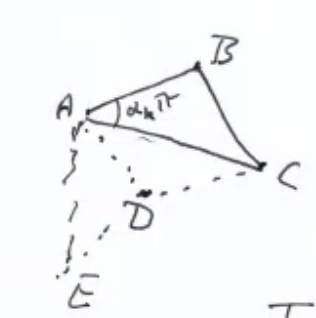
\includegraphics[scale=0.5]{triangle.png}
\end{center}
If we let $B$ reflect to $D$ in $AC$, then the extension of $g$ to $ADC$ will also take real values on $AD$ and $DC$.  Also, the exnteded $g$ will extend by reflection to $ADE$.  The result of the reflection in $AC$ and $AD$ is a rotation by $2 \phi + \psi$, where $\phi + \psi = \alpha_k \pi$, so a rotation by $2 \alpha_k \pi$ and when we preform $2$ reflections, there is no more conjugation of the function.  
\pagebreak
\section{March 1st, 2021}
\subsection{Schwarz Triangle Functions}
We took $G(u) = \int_0^u (u - \xi_1)^{\alpha_1 - 1}(u - \xi_2)^{\alpha_2 - 1}\,du$.  We can take $\xi_1 = 0, \xi_2 = 1$ after scaling.  By reflections, recall that $g$ extends by rotations around a vertex by double the angle.  We get that $\tilde g((z - z_k)e^{2 i \alpha_k \pi} + z_k)$ where $\tilde{g}$ is the extension after one reflection in an adjacent side to $z_k$.  After repeated reflections to an integer number of rotations by $n_k 2 \alpha_k \pi$ and this gets us back to the initial triangle.    In other words, there exists $n_k$ such that $n_l 2\alpha_k \pi = 2\pi$.  Then, $g$ is holomorphic extended to some $\{0 \le |z - z_k| < \epsilon\}$ and if the corresponding point is $\infty$ for $z_k$, then $g$ is meromorphic near $z_k$ with a pole at $z_k$; otherwise it is holomorphic near $z_k$. This happens when $\alpha_k = 1/n_k$, for $n_k \in \N$.  We have $1/n_1 + 1/n_2 + 1/n_3 = 1$ with $n_1 \le n_2 \le n_3$.  This has $3$ solutions $(3 ,3, 3)$, $(2, 4, 4)$ and $(2, 3, 6)$.  We can combine these rotations around vertices to get invariance under shifts.  In the end, $g$ is meromorphic with two periods $g(z + L_k) = g_k$ for $k = 1, 2$.  These are called the Schwarz Triangle Functions.  

\subsection{Conformal Mappings of Rectangles}
We can arrange so that the points are mapped from $-1/k , -1, 1, 1/k$ with $0 < k < 1$ and 
$$G(u) = \int_0^u \frac{du}{\sqrt{(1 - u^2)(1 - k^2 u^2)}}.$$

We consider how $G$ maps the boundary of $\mathbb H$ onto $\R \cup \{\infty\}$.    We have that $G(0) = 0$ and if $K = \int_{-1}^{-1} \frac{du}{\sqrt{(1 - u^2)(1 - k^2 u ^2)}}$, then $G$ maps $[-1, 1]$ to $[-K/2, K/2]$.
When $u \in (1, 1/k)$, then if $K' = \int_1^{1/k}\frac{du}{\sqrt{(u^2 - 1)(1 - k^2 u^2)}}$, then the boundary moves along $[K/2, K/2 + iK']$.  Similarly, $(-1/k, -1)$ goes to $(-K/2 +  iK', -K/2)$.  

Finally, the cases where $(-\infty, -1/k)$ and $(1/k, \infty)$ are symmetric, and the integrand is real, so $\infty$ goes to the middle of $(-K/2 + iK', K/2 + iK')$ and $(-\infty, -1/k)$ goes to $(iK', -K/2 + iK')$.

Then. the inverse function $g$ is real on the boundary of the rectangle and can be extended by reflection.  We find that $g(z + 2K) = g(z)$ and $g(z + 2iK') = g(z)$ and $g$ has a pole at $iK'$ and $K + iK'$ and zeros at $0$ and $K$ so we have poles at $nK + 2(m+1)K' i$and zeros at $nK+2mK'i$.

\pagebreak
\section{March 3rd, 2021}
\subsection{Elliptic Integrals and Functions}
Recall we had a conformal mapping of rectangles given by $$G(w) = \int_0^w \frac{dw}{\sqrt{(1 - w^2)(1 - k^2w^2)}} \quad 0 < k < 1.$$
This is an example of a basic elliptic integral.  More generally, we have 
$$\int_0^w R(w, \sqrt{P(w)}) \,dw$$
where $R$ is a rational function and $P$ is a polynomial of degree $3$ or $4$.  Then, the inverse $g = G^{-1}$ is an elliptic function: doubly periodic and meromorphic.  

\subsection{Tiling the Unit Disk}
We tile the unit disk.  We can tile the disk with a curvilinear triangle with arcs that are geodesics with respect to the hyperbolic metric $\frac{|dz|^2}{(1 - |z|^2)^2}$.  We start with the equilateral triangle with vertices at $i$, $i e^{2\pi i/3}$, and $i e^{-2\pi i 3}$.  If we reflect $i$ with respect to the lower arc, it is mapped to $-i$.  We do the same for the other vertices, and we repeat this to get an Escher-like picture.  All the arcs are the same size with respect to the hyperbolic metric.

Now, if we consider a mapping from the Escher picture to the upper-half plane, it should be invariant under some group of fractional linear transformations, namely $SU(1, 1)$.  So, we look for a way to pass from $SU(1, 1) \to SL(2, \R)$.

We can map our points to $0, 1$ and $\infty$.  (Did you know conformal mappings preserve angles?)  We wish to understand what happens when we reflect about this figure.  When we reflect about the lines, we have the usual reflection.  Before doing this, we precisely describe the connection between the two figures.  Namely, the transformation is given by the cross ratio $(z, ie^{-2\pi i/3}, ie^{2\pi i/3}, i)$(recall that it makes the second point to $0$, third to $1$ and last to $\infty$).  We can understand what's happening by noting that when we map Jordan domains to Jordan domains, they preserve orientation.  Note that $0, 1, \infty$ are counterclockwise.  Writing down the mapping
$$z \mapsto \frac{z - ie^{2\pi i/3}}{z - i} : \frac{ie^{-2\pi i/3} - ie^{2\pi i/3}}{ie^{-2 \pi i/3} - i}.$$

Notice that the second fraction is equal to $e^{\pi i/3} \frac{- \sin(2\pi/3)}{- \sin(\pi/3)} = e^{\pi i /3}$.  This is a counterclockwise rotation by $60^\circ$.  Hence $z \mapsto e^{-\pi i/3} \frac{z - ie^{2\pi i /3}}{z - i}$.  Note that the reflections are given by $z \mapsto - \ol{z}$ for $0, \infty$ $z \mapsto - \ol{z - 1} + 1 = z - \ol{z}$ for $1, \infty$ and $z \mapsto \frac{1/4}{\ol{z - 1/2}}+1/2$.  Composing the rotations, we have $z + z$ and $\frac{z}{2z+1}$.  These give two elements of $SL(2, \R)$, so it follows that $\Gamma$, the free group of invariant transformations generated by these two elements.   This subgroup of $SL(2, \R)$ will also be important later.  

\subsection{Schwarz-Christoffel Revisted}

We will use the Schwarzian derivative, which is similar to the role of the logarithmic derivative in the Schwarz-Christoffel formula. 

Note that the Schwarz-Christoffel formula is given by 
$$F' = c\prod_{k=1}^n (w - w_k)^{-\beta_k}$$
and we get that $$\frac{F''}{F'} = (\log F')' = C + \sum\frac{-\beta_k}{w - w_k}.$$
[The constant might not be necessary.]

The Schwarzian derivative is given by
$$S(f) = \frac{f'''}{f'} - \frac{3}{2}\left (\frac{f''}{f'}\right )^2 = \left (\frac{f''}{f'}\right )' - \frac{1}{2} \left (\frac{f''}{f'}\right )^2.$$

There are some interesting properties of $S(f)$: 
\begin{itemize}
\item $S(f \circ g) = (S(f) \circ g)(g')^2 + S(g)$.
\item For $f(z) = \frac{az+ b}{cz + d}$, $S(f) = 0$.
\item Combining the results, $S(g)$ is invariant under fractional linear transformations.  
\end{itemize}

\pagebreak
\section{March 8th, 2021}
\subsection{Schwarzian Derivative}
Recall that for a fractional linear transformation $f$, $S(f) = 0$, where $S$ is the Schwarzian derivative.  
\begin{proposition} If $S(f) = S(g)$ and $g^{-1}$ exists, then $f = \frac{ag + b}{cg + b}$, with $ad - bc \ne 0$.
\end{proposition}
\begin{proof}
Write $f = h \circ g$.  Then $S(f) = (S(h) \circ g )(g')^2 + S(g)$ and $h = f \circ g^{-1}$, so it follows that $S(h) = 0$.

Then, we claim $S(h) = 0$ implies that $h = \frac{az + b}{cz + d}$.  Let $y = \frac{h''}{2h'} = \frac{1}{2} (\log h' )'$.  Since $S(h) = 0$, we have $y' = y^2$, so $(-1/y)' = 1$, so $y = -\frac{1}{z + c}$.   This implies that $-1/2(\log h')' = (\log(z + c))'$, so $(z + c)^2h' = a$ and $h' = \frac{a}{(z + c)^2}$.  Therefore, $h = b - \frac{a}{z + c}$, which implies the result.
\end{proof}

Given $S(f) =2p$, we wish to recover the function.  

\begin{fact} Given two linearly independent solutions $y_1, y_2$ of $y'' + py = 0$, then $u=  \frac{y_1}{y_2}$ is so that $S(u) = 2p$.
\end{fact} 
\begin{proof}
Given $y_1 = uy_2$, we have $y_2'' + py_2 = 0$ so it follows that 
$$u'' y_2+ 2u'y_2' + uy_2'' + puy_2 = u''(y_2) + 2u'y_2' + u(y'' + py_2) = 0,$$
so it follows that $u''/u' = -2y_2'/y_2$.  

It follows that 
\begin{align*}
S(u) &= (u''/u')' -1/2 (u''/u')^2 \\
&= -2 (y_2'/y_2)' - 1/2 (2y_2'/y_2) \\
&= -2 \frac{y_2''y_2}{y_2^2} \\
&= 2p.
\end{align*}
\end{proof}
\begin{remark} This is well defined because any pair of solutions is connected by a fractional linear transformation, which has a null Schwarzian derivative.  
\end{remark}
\subsection{Curvilinear Polygons}
This case is more complicated than Schwarz Christoffel because the radius of curvature for the arcs between vertices are not uniform.  

We can show that 
$$S(f) = \frac{1}{2} \sum_k \frac{1 - \alpha_k^2}{(z - \alpha_k)^2} + \sum_k\frac{\beta_k}{z - \alpha_k} + \gamma.  $$

Take $n = 3$.  The constants are determined by $\alpha_1, \alpha_2, \alpha_3$(we change this to $\alpha, \beta, \gamma$).  The equation $$u'' + \frac{p}{2}u = 0$$
can be replaced by $$u'' + Pu' + Qu = 0,$$
where we have solutions $y_i \mapsto \sigma(z) y_i$.  The new equation is given by
$$z(1-z) y'' + (c - (a + b + 1)z)y' - aby = 0,$$
which has solutions 
$$c\int_0^1 t^{b-1}(1- t)^{c - b- 1} (1 - zt)^{-a}\,dt,$$
the \textit{hypergeometric functions }.


\begin{proposition} If $\alpha = \beta = \gamma = 0$, then $f(z) = \frac{T(z)}{T(1-z)}$, where $$T(z) = \int_0^1 \frac{dt}{\sqrt{t(1-t)(1-zt)}}.$$
\end{proposition}
\pagebreak
\section{March 10th, 2021}
Recall last time, upon composing reflections where $0, 1, \infty \to 1, \infty, 0$ and extending the half plane, we obtain the modular function $\lambda$ which sends $\frac{az + b}{cz + d} \to \lambda(z)$.  
\subsection{The Modular Function}
\begin{theorem}[Picard] If $g: \C \to \C$ holomorphic such that $|\C \setminus g(\C)| > 1$, then $g$ is constant.  
\end{theorem}
\begin{proof}
We may assume that $\C \setminus g(\C) \supset \{0, 1\}$.  Because of the way that $\lambda$ was extended to $\{\text{im }z > 0\}$ via reflections and fractional linear transformations, one can find $h:\C \to \{\text{im }z > 0\}$ so that $\lambda \circ h = g$.  Note that $\C \setminus \{0, 1\}$ is a covering of $\{Im (z) > 0\}$, and $\lambda$ acts as a simply connected covering map.  Then, there exists a lifting map from $\C \to \{im(z) > 0\}$, which we define as $h$.
\end{proof}

Now, we can apply Liouville's theorem to $h$ since $im(h)>0$.  
\subsection{Analytic Functions}
If $f$ is a meromorphic function with a pole at $b$, it has a Laurent expansion
$$\sum_{k = -N}^\infty c_k(z - b)^k.$$

The term $\sum_{k=-N}^{-1} c_k(z - b)^k$ is called the principle part.  We can develop the theory for meromorphic functions in $\Omega = \C$. 
\begin{theorem}[Mittag-Leffler] Given $b_n \in \C$, $n \in \N$, $\lim_{n \to \infty} |b_n| = \infty$ and principle parts $\sum_{k = -N_n}^{-1} c_k^{(n)}(z - b_n)^k = P_n$, there is a meromorphic function on $\C$ with poles $(b_n)_{n \in \N}$ and principal parts $p_n$ of the Laurent expansions at the poles.
\end{theorem}
\begin{proof}
Roughly, we would want $\sum P_n$, but this might not converge.  If it doesn't converge, we make it convergent by adjusting the function in a way that doesn't change the principal parts.  Define $R_n = \inf_{k \ge n} |b_k|$.  Note that $R_n \uparrow \infty$.  Then, if $R_n > 0$, $\frac{R_n}{2} < |b_m|$ for $m \ge n$.  Since $P_n$ is holomorphic in $R_n\D$, there exist polynomials $p_n$ so that $\|P_n - p_n \|_{R_n/2 \ol{\D}} < 2^{-n}$(assuming $R_n > 0$).

Then $\sum_{m \ge n} (P_m - p_m)$ converges uniformly on compact subsets $R_n/2 \D$ to a holomorphic function on $R_n/2 \D$.  On the other hand, $\sum_{m < n} (P_m - p_m)$ is meromorphic and has the same poles and principles parts as $\sum_{m < n} P_m $.  It follows that $\sum_n (P_n - p_n)$ converges on compact subsets of $\C \setminus \{b_n : n \in \N\}$ with the desired properties.
\end{proof}
\begin{remark} Note that if $f, g$ are mermorphic on $\C$ with poles $b_n$ and principal parts $P_n$, $n \in \N$, then $f - g$ is holomorphic on $\C$.  Also, having $f$, we can get any other merormophic function with these properties by adding an entire function.
\end{remark}
\subsection{Cool Series Expansions}
We will give a series expansion for $\frac{\pi^2}{(\sin{\pi z})^2}$.  Namely, we construct a merormorphic function with the same poles and principle parts and determine the difference.  

Note that the poles are given by the points $z \in \Z$.  The order of the zeros are given by $(\sin{\pi z})' = \pi \cos{\pi z}$.  For $k \in \Z$, $\cos{\pi k} = 1$, so the zeros are simple.  The poles of $\pi^2/(\sin{\pi z}^2)$ are order $2$ at $n \in \Z$.  Note that it is periodic of period $1$.  To compute the principle part, we compute the principal part at $z = 0$.  Note that $\pi^2/(\sin{\pi z}^2)$ is an even function with a pole of order $2$ so the principle part is even, so it is $a/z^2$, where
$$a = \lim_{z \to 0} \frac{\pi^2}{(\sin{\pi z})^2} z^2 = (\lim_{z \to 0} \frac{\sin{\pi z}}{\pi z})^{-2} = 1.$$

The principle part at $z = n$ is thus given by $1/(z - n)^{-2}$.  Note that $\sum_{n \in \Z} \frac{1}{(z - n)^2}$ converges uniformly on compact subsets of $\C \setminus \Z$.   

It follows that 
$$\sum_{n \in \Z} \frac{1}{(z - n)^2} - \frac{\pi^2}{(\sin{\pi z})^2}$$
is holomorphic on $\C$.  Next time, we prove that it is exactly $0$.
\pagebreak
\section{March 15th, 2021}
\subsection{Cool Series Expansion, continued}
\begin{theorem}[Mittag-Leffler] Given $b_n \in \C$, $n \in \N$, $\lim_{n \to \infty} |b_n| = \infty$ and principle parts $\sum_{k = -N_n}^{-1} c_k^{(n)}(z - b_n)^k = P_n$, there is a meromorphic function on $\C$ with poles $(b_n)_{n \in \N}$ and principal parts $p_n$ of the Laurent expansions at the poles.
\end{theorem}
We applied this to find a series expansion of $\frac{\pi^2}{\sin{\pi z}^2}$.  We reduced it to an entire function $h = f_1 - f_2$ holomorphic with $f_1(z + 1) = f_1(z)$, $f_2(z + 1) = f_2(z)$, which implies that $h(z+1) = h(z)$.  We show that $h = 0$ exactly.  We do this by showing it is a bounded function which implies that it is zero by the Louiville theorem.  
\begin{proof}
Let $A(R) = \{|Im(z)| \ge R\} $We claim that $\|h\|_{A(R)} \to 0$ as $R \to \infty$.  We do this by showing it for both $f_1$ and $f_2$.  Note that 
$$|\sin \pi(x + iy)| \ge \frac{1}{2} |e^{\pi y} - e^{-\pi y}|,$$
so it follows that 
$$\left\| \frac{\pi^2}{\sin{\pi z}^2}\right\|_{A(R)} \le \frac{4\pi^2}{|e^{\pi R} - e^{-\pi R}|} \xrightarrow{R \to \infty} 0.$$

For $f_2$, $|Im(z)| \ge R$ so $$|\sum (z-n)^{-2}| \le \sum |z - n|^{-2} \le \sum ((x-n)^2 + R^2)^{-1} \le R^{-2} + \sum (n^2 + R^2)^{-1} \xrightarrow{R \to \infty} 0.$$

It follows that $$\|h\|_\C \le \|h\|_{|Re(z)|\le 1/2} \le \|h\|_{|z| \le R} + \|h\|_{|Im(z) \ge R/2|} < \infty.$$

Then $h = C$.  Since $|C| = \|h\|_{Im(z) \ge R} \to 0$, it follows that $C = 0$.  Therefore, $$\frac{\pi^2}{\sin{\pi z}^2} = \sum_{n \in \Z} \frac{1}{(z - n)^2}.$$
\end{proof}

Can we make sense of $\sum_{n \in \Z} \frac{1}{z-n}$?
We can write
$$\frac{1}{z} + \sum_{n \in \Z \setminus \{0\}} \frac{1}{z-n} + \frac{1}{n}.$$
The counterterms are suitable because
$\frac{1}{z-n} + \frac{1}{n} = \frac{z}{n(z-n)}$, so for $R > 0$, $|n| \ge R+1$implies that
$$\|z/(n(z-n))\|_{R\ol\D} \le \frac{R}{|n|(|n| - R)},$$
so it follows that 
$$\sum_{|n| \ge R + 1} \frac{R}{|n|(|n| - R)} < \infty.$$

Alternatively, note that $\sum_{0 < |n| < N} 1/n  = 0$ so 
$$\lim_{N \to \infty} \sum_{|n| \le N} \frac{1}{z-n} = \frac{1}{z} + \sum_{n \in \Z \setminus \{0\}} \frac{1}{z-n} + \frac{1}{n}.$$
If we denote $g_n(z) = \sum_{|n| \le N} \frac{1}{z-n}$, this is called the Eisenstein summation by Andre Weil, the author of the Weil Conjectures.  

Then $g_N(z)$ is uniformly convergent on compact subsets of $\C \setminus \Z$.  From this, we can compute $g_N'(z)$ which is uniformly convergent on compact subsets of $\C \setminus \Z$.  Furthermore,
$$g_N'(z) = -\sum_{|n| \le N} \frac{1}{(z-n)^2} \to -\frac{\pi^2}{\sin{\pi z}^2}.$$
Note that this is also the derivative of $\pi\cot{\pi z}$, so it follows that $g = \pi \cot{\pi z} + C$.

We can show the $C = 0$ using the fact that $\cot$ is odd, namely, $g(z) = -g(-z)$(the symmetric sums are all odd functions). 
\subsection{Infinite Products}
A polynomial with zeros $z_1, \dots, z_n$ is $P(z) = \prod_{1 \le k \le n}(z - z_k)$.  Given a sequence $z_1, z_2, \dots$ with $|z_k| \to \infty$, can we find a holomorphic function $f:\C \to \C$ with these zeros?  This is a theorem of Weierstrass.  

\begin{remark} One reason why this can be strange is because we can approach numbers from different directions and obtain different convergence behavior.  
\end{remark}
Let $z_k \in \C \setminus \{0\}$.  
\begin{definition} $\prod_{k \ge 1} z_k$ is convergent if $\lim_{n \to \infty} \prod_{k=1}^n z_k$ exists and is nonzero.  We denote $\log z$ if $z \ne 0$ the set $\{a \in \C: e^a = z\}$ and by $Log(z)$, the number $a \in \R + i(-\pi, \pi]$ so that $e^a = z$.  Similarly, $\arg z = Im(\log z)$ and $Arg(z) = Im(Log(z))$.
\end{definition}
\begin{fact} $\prod_{k \ge 1} z_k$ convergent if and only if $\sum_{k \ge 1} Log(z_k)$ is convergent.  
\end{fact}

\begin{fact} $\prod_{k \ge 1} z_k$ convergent, then $z_k \to 1$.  
\end{fact}

\begin{proof}
If we put $P_n = \prod_{1 \le k \le n} z_k$ and $S_n = \sum_{1 \le k \le n} Log(z_k)$, then $\lim_{n \to \infty} S$, then $e^S = \lim_{n \to\ infty} e^{S_n} = \lim_{n \to \infty} P_n$, so $\lim_{n \to \infty} P_n = e^s \ne 0$.

Conversely, suppose $\lim_{n \to \infty} P_n = P \ne 0$.  Then $P_n/P \to 1$, so $\log(P_n/P) \to 0$.  Then $Log(P_n/P) = S_n - Log(P) + 2\pi i h_n$ for some $h_n \in \Z$.  Note that 
$$2\pi i(h_{n+1} - h_n) = Log(P_{n+1}/P) - Log(P_n/P) - Log(z_{n+1}),$$
and the right hand side is $0$ for large $n$.  Indeed, there is an $\epsilon > 0$ so that $|a - 1| < \epsilon$, $|b - 1| < \epsilon$ so we have $Log(ab) = Log(a) + Log(b)$, and we can show that $h = \lim h_n$ exists which implies the convergence.  
\end{proof}
\begin{definition} $\prod_{k \ge 1} z_k$ is absolutely convergent if $\sum_{k \ge 1} |Log(z_k)| < \infty$.
\end{definition}
\begin{fact} $\prod_{k \ge 1} z_k$ is absolutely convergent if and only if $\sum_{k \ge 1} |z_k - 1| < \infty$.  
\end{fact}
\begin{proof}
It follows from noting that the derivative of $Log(z)$ at $1$ is $1$.  
\end{proof}
This allows us to permute terms in products when we have absolute convergence.  
\pagebreak
\section{March 17th, 2021}
\subsection{Weierstrass Theorem}
Our goal is to construct holomorphic functions with prescribed zeros on $\C$.  We have $a_n \in \C$ and $|a_n| \to \infty$(so that we don't have accumulation points).  A zero of order $m$ at zero would be handled by $z^m$ and $a_n \ne 0$.  This gives $z^m \prod_{n=1}^\infty \left (1 - \frac{z}{a_n}\right )$, so that when $a_n$ becomes large, the term becomes small.  This issue is that this may not converge. 

\begin{remark} Take $|\zeta| < 1$.  Then $1 - \zeta \ne 0$ and $Re(1 - \zeta) > 0$, $Arg(1 -\zeta) \in (-\pi/2, \pi/2)$.  The series expansion of $\log(1 - \zeta)$ is $-\sum_{k \ge 1} \zeta^k/k$ and we replace with $Log$ so that it uniformly converges.  
\end{remark}
To make $\sum_{n \ge 1} Log(1 - z/a_n)$ uniformly convergent on compact subsets, we take $R_n = \inf_{k \ge n} |a_k|$ and choose a polynomial $p_n$ so that $$\|Log(1 - z/a_n) - p_n(z)\|_{R_n/2 \ol \D} M 2^{-n}.$$

We can choose $p_n(z) = -\sum_{k=1}^{k_n} (z/a_n)^k/k$ where $k_n$ so that $$\sum_{k > k_n} |(R_n/2 )/ a_n|^k 1/k < 2^{-n}.$$
Then, $|z| \le R_n/2$ implies that the choice of $k_n$ is correct.    Now, we define $g_n(z) =Log(1 - z/a_n) - p_n(z) = Log(1 - z/a_n) + \sum_{k=1}^{k_n} (z/a_n)^k /k$.  It follows that $\|g_k\|_{R_n/2\ol\D} < 2^{-k}$ for $k \ge n$ so it follows that $\prod_{k \ge n} e^{g_k}$ is convergent so that $\|e^{g_k} - 1\|_{R_n/2 \ol \D} < e^{2^{-k}} -1$ and $\prod_{k \ge n} e^{g_k}$ converging uniformly on $R_n/2 \ol \D$.  Thus, 
$$P = z^m \prod_{n=1}^\infty (1 - z/a_n) e^{z/a_n + \dots + z^{k_n}/a_n^{k_n} \cdot 1/k_n}$$
is uniformly convergent(after omitting the zero terms) on a given compact set of $\C$.   Then $P$ is a holomorphic function on $\C$ with zeros $a_n$(with multiplicities respected).  If $f$ is a holomorphic function on $\C$ with the same zeros then $f/P$ and $P/f$ are holomorphic entire functions so $f/p = e^g$ for some holomorphic $g$ on $\C$.    Hence, we have proved the following theorem:
\begin{theorem}[Weierstrass] Given $a_n \in \C$, $|a_n| \to \infty$, there exists a holomorphic function on $\C$ with precisely these zeros.  Every holomorphic function on $\C$ with these zeros, $a_n \ne 0$ and zero of multiplicity $m$ at $0$ is $$f(z) = z^m e^{g(z)} \prod_{n \ge 1} (1 - z/a_n) \exp(z(/a_n + \dots + (z/a_n)^{k_n}) \cdot 1/k_n)$$
for some $k_n \ge 0$ and $g$ holomorphic on $\C$.
\end{theorem} 
\begin{corollary} If $f$ is meromorphic on $\C$, then there are $f_1, f_2$ holomorphic so that $f = f_1/f_2$.
\end{corollary} 
\begin{proof}
The Weierstrass theorem gives $f_1$ with some zeros as $f$ and $f_2$ with zeros same as the poles of $f$, so $f_1/f_2 = e^g f$, with $g$ holomorphic on $\C$.  Replace $f_1$ with $f_1e^{-g}$ so that $f_1/f_2 = f$.
\end{proof}

\subsection{Cohomology Aspects}
We remarked before that Mittag-Leffler and Weierstrass relate to sheaf cohomology.  Roughly, a sheaf of sets is defined as follows.  We have a topological space, as for each open set, we have a functor mapping this to a set of real valued continuous functions on the set.  If we take a two open sets with $A \subset B$ then every continuous function on $B$ restricts to a continuous function on $A$, so we have a contravariant functor.   We also want the property that if we have sets $U_i, U_j$ open and if the functions on $U_i \cap U_j$ give the same thing, then we have some global function with the same properties.  We can also take a different Abelian category instead of a set.  We can define a cohomology on this via Cech Cohomology: given open sets, we take the Cech cocycle so that with the intersection of two sets, we have two functions with are compatible with each other on the intersection.  

The problems that are solved by Mittag-Leffler and Weierstrass solve cohomological problems with the sheaf of holomorphic functions with additive structure and the sheaf of nonvanishing holomorphic functions that don't vanish, which is a sheaf of Abelian groups with respect to multiplication.  

Consider Mittag-Leffler.  We have $P_k$ principle parts with poles of $a_k$.  Take covers $(U_i)_{i \in I}$ covers of $\C$ with bounded open sets.   Define $\phi_i = \sum_{\{k: a_k \in U_i\}} P_k$, a finite sum, and $\phi_i$ meromorphic in $U_i$.  Then, $\phi_i - \phi_j = h_{ij}$ is holomorphic on $U_i \cap U_j$.   One can verify that this $h_{ij}$ satisfies the cocycle properties. If we can find $h_i$ holomorphic on $U_i$ so that $h_i - h_j = h_{ij}$ on $U_i \cap U_j$, the $(\phi_i - h_i)\vert_{U_i \cap U_j} = (\phi_j - h_j)_{U_i \cap U_j}$(this is a coboundary condition).  But this is exactly solving the Mittag-Leffler problem.  

This is the Cousin problem(additive): given $h_{ij}$ holomorphic on $U_i \cap U_j$, $h_{ij} + h_{jk} + h_{ki} = 0$ on $U_i \cap U_j \cap U_k$ and $h_{ij} = -h_{ji}$ on $U_i \cap U_j$.  We want to find $h_i$ holomorphic on $U_i$ so that $h_i - h_j = h_{ij}$ on $U_i \cap U_j$.  Note that Cousin problem has a solution implies Mittag-Leffler.  

For the Weierstass Theorem, we have $\phi_i = \prod_{k | a_k \in U_i}(z- a_k)$, and $\phi_i/\phi_j = g_{ij}$ holomorphic, invertible on $U_i \cap U_j$.  We need $g_i$ holomorphic invertible on $U_i$ so that $g_i/g_j = g_{ij}$ on $U_i \cap U_j$. Then, $\phi_i/g_i = \phi_j/g_j$ on $U_i \cap U_j$ and there is $f$ holomorphic on $\C$ so that $f\vert_{U_i} = \phi_i/g_i$.  

This is the Cousin problem(multiplcative): given $g_{ij} \ne 0$ holomorphic on $U_i \cap U_j$ with $g_{ij} = g_{ji}^{-1}$, $g_{ij}g_{jk}g_{ki} = 1$ on $U_i \cap U_j \cap U_k$.  We wish to find $g_i$ holomorphic and nonzero on $U_i$ so that $g_i/g_j = g_{ij}$ on $U_i \cap U_j$.
\pagebreak
\section{March 29th, 2021}
\subsection{Infinite Products}
Recall that given $a_n \ne 0$, $|a_n| \to \infty$, $m$ order of zero at $0$, there are $k_n \ge 0$ integers so that $$P(z) = z^m \prod_{n \ge 1} (1 - z/a_n) e^{(z/a_n + \dots + (z/a_n)^{k_n} )( 1/k_n)}$$
is a uniformly absolutely convergent product that gives a holomorphic function with prescribed zeros.  Any other holomorphic function with these zeros is $e^{g(z)}P(z)$ for some holomoprhic function $g$ on $\C$.

How do we choose $k_n$?   If we take a subsequence of the $k_n$ so that $\sum_j 1/|a_{n_j}| < \infty$, then we can choose $k_{n_j} = 0$.  We can also set any finite number of them to $0$ without issues.  If we assert that all the $k_n$'s must be equal, what is the proper choice of $k_n = k$?  These are called the \textbf{canonical products}.  Furthermore, if $f: \C \to \C$ is holomophic and $f = e^{g(z)} P(z)$, $f$ has \textbf{finite genus} if $P$ is a canonical product and $g$ is a polynomial.  

In the proof of the Weierstrass theorem, we had 
$$\|Log(1 - z/a_n) + \sum_{m=1}^{k_n} (z/a_n)^m /m \|_{\rho \ol \D} \le \sum_{m > k_n} (\rho/|a_n|)^m /m,$$
which is convergent for $|a_n| > \rho$.

So $\sum_n \sum_{m>} (\rho/|a_n|)^m 1/m < \infty$, which implies convergence of the canonical product.  Howevr, note that only the first term matters since
$$(\rho/|a_n|)^{h+1}/(h+1) \le \sum_{m > h} (\rho/|a_n|)^m/m \le (\rho/|a_n|)^{m+1}/(m+1) \frac{1}{1-\rho/a_n}.$$
Since $\rho < |a_n|$, our series converges properly.  It follows that $\sum_n 1/|a_n|^{h+1} < \infty$ implies the convergence of the canonical product.  
We define $genus(P) = \inf \{h\in \Z, h \ge 0| \sum_n 1/|a_n|^{h+1} < \infty\}$.  
\begin{definition} If $f: \C \to \C$ has finite genus, we define $genus(f) = \max(\deg g, genus(P))$.
\end{definition}
\begin{itemize}
\item If $f$ is genus zero, then $f(z) = Cz^m \prod_{n \ge 1} (1 - z/a_n)$ with the assumption that $\sum 1/|a_n| < \infty$.  
\item  If $f$ is genus $1$, then we have $f(z) = Cz^m e^{\alpha z} \prod_{n \ge 1} (1 - z/a_n)e^{z/a_n}$ and $\sum 1/|a_n| = \infty$ but $\sum 1/|a_n|^2 < \infty$ OR we have that $f(z) = Cz^m e^{\alpha z} \prod_{n \ge 1} (1-z/a_n)$ for $\alpha \ne 0$ and $\sum 1/|a_n| < \infty$.  
\item Take $f(z) = \sin{\pi z}$, with zeros at the integers.  Then, $\sum_{n \in \Z \setminus \{0\}} 1/|n| = \infty$, $\sum_{n \in \Z \setminus \{0\}} 1/n^2 < \infty$.  We can consider the canonical product $P = z \prod_{n \in \Z \setminus \{0\}}(1-z/n)e^{z/n}$, which is of genus 1.  Then, $\sin \pi z = e^g z \prod_{n \in \Z \setminus \{0\}}$.  Recall that the logarithmic derivative gives
$$\pi \cot{\pi z} = g' + 1/z + \sum_{n \in \Z^\times} (1/n + 1/(z-n)).$$
We recall that the right term is $g' + \pi \cot{\pi z}$, so it follows that $g' = 0$ and $g = C$.  We can solve for $C$ by noting that $e^C z \prod_{n \in \Z^\times }(1 - z/n)e^{z/n} = \sin{\pi z}$.  We can divide by $z$ and taking limits, we obtain that $e^C = \pi$, so it follows that $C = \log \pi$.  It follows that $\sin \pi z = \pi z \prod_{n \in \Z^\times} (1-z/n) e^{z/n}$.  We could also write this as $\pi z \prod_{n \ge 1} (1 - z^2/n^2) = \sin{\pi z}$.  
\end{itemize}

\subsection{Hadamard's Theorem}
We can relate to the growth of a holomorphic function $f: \C \to \C$ and the order of the growth 
$$\rho - \limsup_{R \to \infty} \frac{\log \log \|f\|_{R\ol{\D}}}{\log R}.$$
We could also write
$$\rho = \inf \{m \ge 0: |f(z)| \le Ce^{C|z|^m}\}.$$
\begin{theorem}[Hadamard] If $\rho$ order of growth of $f$, $h$ genus of $f$, then $\rho \in [h, h+1)$.
\end{theorem}
Next time, we use the construction of the Gamma function and we follow the proof of Ahlfors which considers the zeros.  We somehow end up with the Gamma function $G(z-1) = ze^{\gamma(z)}G(z)$ for an entire function $\gamma$.  

\pagebreak
\section{March 31st, 2021}
\subsection{The Gamma Function}
Consider the canonical product for the zeros $\{-1, -2, \dots\}$, which leads to
$$G(z) = \prod_{n \ge 1} (1 + z/n) e^{-z/n}.$$
$G(z-1)$ has zeros $\{0, -1, -2, \dots\}$, hence $G(z-1)=ze^{\gamma(z)}G(z)$ for an entire function $\gamma$.

If we take the logarithmic derivative, we obtain
\begin{align*}
\sum_{n \ge 1} \frac{1/n}{1 + (z-1)/n} - 1/n &= \gamma'(z) + 1/z + \sum_{n \ge 1} (1/n / (1 + z/n) - 1/n),
\end{align*}
and from here, we can obtain $\gamma'(z) = 0$ via a telescoping series.  Hence, $\gamma(z) = \gamma$, for a constant $\gamma$, which happens to be the famous Euler-Mascheroni Constant.  IT follows that $G(z-1) = e^{\gamma}z G(z)$.  If we define $H(z) = e^{\gamma z} G(z)$, then it follows that $H(z-1) = zH(z)$.

Take $z=1$.  We have $G(0) = e^\gamma G(1)$ and $G(0) = 1$ so $1 = e^\gamma \prod_{n \ge 1} (1 + 1/n) e^{-1/n}$.  Taking the logarithm, we obtain $$-\gamma = \lim_{N \to \infty} \sum_{n=1}^N (\log (n+1) - \log n) - 1/n,$$ but this gives a telescoping sum with exactly the limit $\lim \log(N) - (1 + \dots + 1/N)$.  This is exactly the Euler-Mascheroni constant.  

Define $\Gamma(z) = \frac{1}{zH(z)}$.  Then, $$\Gamma(z+1) = \frac{1}{(z+1)H(z+1)} = \frac{1}{H(z)} = \frac{z}{zH(z)} = z\Gamma(z).$$
From the definition of $\Gamma$, it follows that $\Gamma(z)$ is a meromorphic function with poles at $-\N$, no zeros, and $\Gamma(z+1) = z\Gamma(z)$.

Writing this explicitly, we have
$$\boxed{\Gamma(z) = z^{-1} e^{-\gamma z}\prod_{n \ge 1}(1 + z/n)^{-1} e^{z/n}}.$$

If we take $G(-z) z gG(z) = z \prod_{n \in \Z^\times} (1-z/n)e^{z/n} = \frac{\sin{\pi z}}{\pi}.$  Then, noting that $G(z) = e^{-\gamma z}H(z) = \frac{e^{-\gamma z}}{z\Gamma(z)}$, we find that 
$$\frac{\pi}{\sin{\pi z}} = \Gamma(z) \Gamma(1-z).$$

\subsection{Particular Values of $\Gamma$}
It is clear that $\Gamma(1) = \lim_{z \to 0} \Gamma(1 + z) = \lim_{z \to 0}z\Gamma(z) = 1$.  So we obtain the value of $\Gamma(n)$ for each $n \in \N$, namely, $\Gamma(n+1) = n!$, which is clear by induction.

Note that 
$$\Gamma(1/2)^2 = \Gamma(1/2)\Gamma(1 - 1/2) = \frac{\pi}{\sin{\pi/2}} = \pi.$$

It follows that 
$$\Gamma(n + 1/2) = \sqrt{\pi} \frac{1}{2} \frac{3}{2} \dots (n - 1/2),$$
for $n \ge 0$.

\subsection{Alternate Definition of $\Gamma$}
Take $I(z) = \int_{0}^\infty t^{z-1} e^{-t}\,dt$.      We will show that $I(z)$ extends to a meromorphic function on $\C$ which is exactly $\Gamma(z)$.

We can write $I(z) = I_1(z) + I_2(z)$ where we take the same integrals but from $0$ to $1$ and $1$ to $\infty$ respectively.  Note that $|t^{z-1}e^{-t}| = t^{x-1} e^{-t}$ if $z = x+iy$.It follows that $$\int_{0}^1 |t^{z-1}e^{-t}|\,dt = \int_{0}^1 t^{x-1} e^{-t}\,dt \le \int_{0}^1 t^{x-1}\,dt.$$
This is finite whenever $x > 0$, so $I_1(z)$ is defined if $Re(z) > 0$. $I_2$ is "very" convergent, the exponential decay handles the polynomial term.

 We can show that $I_1$ holomorphic function on $\{Re(z) > 0\}$.  This requires the machinery of the Dominated Convergence Theorem, but roughly we differentiate under the integral sign and pass the derivatives onto the exponential terms.  We can also show the second integral is defined for $z \in \C$ and holomorphic via differentiation under the integral.
 
 We can show the recurrence relation $I(z+1) = zI(z)$ for $Re(z) > 0$ via integration by parts with an approximating integral $\int_a^b t^z e^{-t}\,dt$ and taking the limit as $a \downarrow 0$ and $b \uparrow \infty$, where the boundary terms vanish.  We can also show directly that $I(1) = 1$, so $I(z)$ and $\Gamma(z)$ satisfy the same recurrence relation if $Re(z) > 0$.
 
 Now, define $\psi(z) = \frac{I(z)}{\Gamma(z)}$, which is well defined $Re(z) > 0$, is holomorphic, and $\psi(z+1) = \psi(z)$. 

\pagebreak
\section{April 5th, 2021}
\subsection{Gamma Function, continued}
Last time, we defined $\psi(z) = \frac{I(z)}{ \Gamma(z)}$ which is a holomorphic function on the real half place with the relation $\psi(z + 1) = \psi(z)$, where $I(z)$ is the integral formulation of the Gamma function.

We begin by taking $A(y) = \sup_{1 \le x \le 2} |\psi(x + iy)|$.  Then,
$$\sup_{1 \le x \le 2} |I(x + iy)| \le \sup_{1 \le x \le 2} \int_0^\infty t^{x-1} e^{-t}\,dt = C < \infty.  $$

Then,
\begin{align}
\sup_{1 \le x \le 2} \frac{1}{|\Gamma(x + iy)|} &\le |2 + iy| e^{2\gamma} \sup_{1 \le x \le 2} |\prod_{n \ge 1} (1 + (i + iy)/n) e^{-x/n}| \\
&\le C(1 + |y|) \sup_{1 \le x \le 2} \prod_{n \ge 1} |1 + x/n| |1 + iy/n| e^{-x/n} \\
&\le C(1 + |y|) \cdot \prod_{n \ge 1} (1 + y^2/n^2)^{1/2} 
\end{align}
using the inequality $a > 0 \implies |1 + a + ib| \le |1 + a| |1 + ib|$ in (2) and $(1 + x/n)e^{-x/n} \le 1$ for $x > 0$ in (3).

Then, recall that $\frac{\sin{\pi z}}{\pi z} = \prod_{n \ge 1} (1 - z^2/n^2)$, so it follows by taking $z = iy$ that if $|y| \ge 1$,
\begin{align*}
\sup_{1 \le x \le 2} \frac{1}{|\Gamma(x + iy)|} &\le C(1 + |y|) |\sin{\pi i y}/(\pi i y)|^{1/2} \\
&\le C(1 + |y|) ((e^{\pi|y|} + e^{-\pi |y|})/(2 \pi |y|))^{1/2} \\
&\le C(1 + |y|) e^{\pi/2 |y|} \\
&\le C e^{\pi |y|}
\end{align*}


It follows that $A(y) \le C e^{\pi |y|}$.  Since $\psi(z+ 1) = \psi(z)$, we plug in $\psi(\log w / 2\pi i)$ for $w \in \C \setminus \{0\}$ which does not depend on the choice of branch of the logarithm.  Hence, $\psi(\log w/2\pi i) = h(w)$ is a holomorphic function since $\log$ is locally invertible.  

Then, $h(e^{2\pi i z}) = \psi(z)$ and if $z = x + iy$, $e^{\pi|y|} = \max (e^{\pi y}, e^{-\pi y}) = \max (|e^{2\pi i z}|^{1/2}, |e^{2\pi i z}|^{-1/2})$.

Hence, $|h(w)| \le C (|w|^{1/2}, |w|^{-1/2})$ for $w \in \C \setminus \{0\}$.

Then, the Laurent expansion of $h$ is 
$$h(w) = \sum_{n \in \Z} c_n w^n$$
and $$c_n = (2\pi i)^{-1}\int_{|w| = R} w^{-n-1} h(w) \,dw.$$

From the bounds on $h$, we obtain
$$|c_n| \le 1/2\pi 2\pi R R^{-n-1} \max(R^{1/2}, R^{-1/2}) = C R^{-n} \max(R^{1/2}, R^{-1/2}).$$

If $n > 0$, then $|c_n| \le C \lim_{R \to \infty} R^{-n+1/2} = 0$.  Otherwise,  we take $|c_n| \le C \lim_{R \to 0} R^{|n| - 1/2} = 0$.  So $h = c_0$ and $\psi$ is constant.  It follows that $I(z) = c\Gamma(z)$ for $Re(z) > 0$ and $\Gamma(1) = 1 = I(1)$ implies that $c = 1$.

Hence, we obtain
$$\Gamma(z) = \int_0^\infty t^{z-1} e^{-t}\,dt \quad Re(z) > 0.$$
\subsection{Complex Stirling Formula}
$\Gamma(z) = \sqrt{2\pi} z^{z- 1/2} e^{-z} e^{J(z)}, Re(z) > 0$ where
$$J(z) = \frac{1}{\pi} \int_0^\infty \frac{z}{\eta^2 + z^2} \log \frac{1}{1 - e^{-2 \pi \eta}} \, d\eta.$$

If $|z| \to \infty$, $z \in \{Re(z) \ge c\}$, $c > 0$, then $J(z) \to 0$.

\subsection{Gamma function Heuristics}
If $f: \R \to \C$ is a function so that $\int_\R |f(t)| \, dt < \infty$, then one can define $\int_\R f(t) e^{ixt}\,dt = \mathcal{F} f(x)$.  This is the Fourier transform, which is a special case of more general transforms.  More generally, we have an abelian group $G$ with the topology compatible with the group structure(this is generally locally compact Hausdorff).  An integral $\int_G f(g) \,dg$ for functions $f:G \to \C$ so that the integral is invariant under translations: namely
$$\int_G f(g)\,dg = \int_G f(g_1 g) \,dg.$$

The map $f \mapsto \int_G f(g)\,dg$ is a linear map.  We could hence define the general Fourier transform as $$\int_G f(g) \chi (g) \,dg = \mathcal Ff(\chi),$$
where $\chi: G \mapsto \{|z| = 1\}$ is a continuous group homomorphism.  

We can also define a complex Fourier transform 
$$\int_\R f(t) e^{zt} = \mathcal F f(z), z \in \C$$
We can also generalize the Haar Fourier transform by taking homomorphisms $\chi : G \to \C^\times$.  

If we take $G = ((0, \infty), \cdot)$ positive numbers with multiplication, this is isomorphic to $(\R, +)$ with an isomorphism given by $t \mapsto e^t$ forward and $\lambda \mapsto \log \gamma$ backwards.  

The continuous homomorphisms from $(0, \infty) \to \C^\times$ are $\chi(\lambda) = \lambda^z$, $z \in \C$.

The invariant integral is 
$$\int_0^\infty f(\lambda) \frac{d\lambda}{\lambda}.$$

The Mellin transform is the complex Fourier transform on $((0, \infty), \cdot)$, namely
$$\int_0^\infty \lambda^z f(\lambda )d\lambda/\lambda = \int_0^\infty \lambda^{z-1} f(\lambda) d\lambda.  $$

To obtain $I(z)$, we take $f(\lambda) = e^{-\lambda}$.  Then $t \mapsto e^{-t}$ is a homomorphism from $(R, +) \to \C^\times$.  We can identify $(0, \infty)$ with the squares of $\R^\times$.

This process can be generalized.  We will mention this next time.
\pagebreak
\section{April 7th, 2021}
\subsection{Mellin Transform}
Some examples of Haar Measures:
\begin{itemize}
\item For $G = \R$, the corresponding Haar Measure is $\int_\R f(t)\,dt$. 
\item For $G = \Z$, $\sum_{n \in \Z} f(n)$.
\item For $G = \{|z|  = 1\}$, $\int_0^1 f(e^{2\pi i t})\,dt$.
\item $G = (\R^+, \cdot) \cong (\R, +)$, we have $\int_0^\infty f(\lambda) \frac{d\lambda}{\lambda}$.
\end{itemize}

Last time, we mentioned that if we take characters $\chi: (0, \infty) \to \C^\times$ of the form $\chi(t) = t^z$, then,
$$\mc F f(\chi) = \int_0^\infty t^{z-1} f(t)\,dt = \int_0^\infty f(t) t^z dt/t.$$

When $f(t) = e^{-t}$, we exactly recover the Gamma function:
$$\Gamma(z) = \mc F f(\chi) = \int_0^\infty t^{z-1} e^{-t}\,dt.$$

What if we take a more general character $f(t) = e^{-\lambda t}$.  If we assume $\lambda > 0$, then the integral
$$\int_0^\infty t^z e^{-\lambda t} dt/t = \int_0^\infty (t/\lambda)^z e^{-\lambda(t/\lambda)}dt/t = \lambda^{-z} \int_0^\infty t^z e^{-t}dt/t = \lambda^{-z} \Gamma(z).$$ 

Replace $e^{-\lambda t}$ by a sum $g(t) = \sum_n c_n e^{-\lambda_n t}$ with $\lambda_n \uparrow \infty$, $\lambda_n > 0$.

Formally, the Mellin Transform of $g(t)$ is 
$$\int_0^\infty t^z \sum c_n e^{-\lambda_n t} dt/t = \Gamma(z) \sum_n c_n \lambda_n^{-z}.$$

\subsection{Riemann Zeta Function}
Take $g(t) = \sum_{n \ge 1} e^{-nt}$.  Note that $g(t) = \frac{1}{e^t - 1}$.  The Mellin transform of this is 
$$\int_0^\infty \frac{t^z}{e^t - 1} \frac{dt}{t} = \Gamma(z) \sum_{n \ge 1} n^{-z}= \Gamma(z) \zeta(z).$$

Note that $(e^t - 1)^{-1} \sim t^{-1}$ as $t \downarrow 0$ so we need $Re(z) > 1$ for convergence.  More generally, we could use $g(t) = \sum_{n \ge 1} e^{-n^k t}$ for an integer $k > 1$, which has Mellin transform $\Gamma(z) \zeta(kz)$.

We will explain the $k = 2$ relation, namely
$$\int_0^\infty \sum_{n \ge 1} e^{-n^2 t} dt/t = \Gamma(z) \zeta(2z),$$
which holds if $Re(z) > 1/2$.

The convergence requires $\sum_{n \ge 1} e^{-n^2 t} \le C/\sqrt{t}$ for $t > 0$.  We can estimate this by comparing with the corresponding integral, which gives the desired result.  We replace with the theta function $\theta(t) = \sum_{n \in \Z} e^{-\pi n^2 t}$ so that $\theta(t) = 2\psi(t) + 1$, where $\psi(t) = \sum_{n \ge 1} e^{-\pi n^2 t}$.

Note the following fact $\theta(t) = \theta(1/t)/\sqrt{t} $ if $t > 0$.  The key to proving this is the Poisson summation formula, namely
$$\sum_{n \in \Z} f(n) = \sum_{n \in \Z} \mc F f(n).$$

We apply this to $e^{-ct^2}$ for some $c$.  

\pagebreak
\section{April 12th, 2021}
\subsection{Poisson Summation Formula}
We were proving $\Theta(t) = 1/\sqrt{t}\Theta(1/t)$, $t > 0$ where $\Theta(t) = \sum_{n \in \Z} e^{-\pi n^2 t}$.  This is done via the Poisson Summation formula.  

We first present the proof of the Poisson Summation formula.   We have an exact sequence
$$0 \to \Z \to \R \to \R/\Z \to 0.$$
The map from functions on $\R$ to a function on $\R / \Z$ is given by $f \mapsto \sum_{n \in \Z} f(t + n)$.  If we take a Fourier Transform on $\R / \Z$, then $\R/\Z \cong \{|z| = 1\}$ whose characters are $t \mapsto e^{2\pi i t}$.  Then, $G:[0, 1) \to \C$ we have
$$\mc F_{\R/\Z} G(k) = \int_0^1 G(t) e^{-2\pi i k t}\,dt.$$

Note that $$c_k = \mc F_{\R / \Z} F(k) = \int_0^1 F(t) e^{-2 \pi i k t} \,dt = \mc F_{\R} f(k).$$

Then,
$$F(0) = \sum_{n \in \Z} c_k e^{2\pi i k \cdot 0} = \sum_{n \in \Z} c_k.$$
So it follows that 
$$\sum_{n \in \Z} f(n) = \sum_{k \in \Z} \mc F_{\R} f(k).$$

First, we put conditions on $F$ so that the computation for $c_k$ is rigorous.  It is clear that we need at least $F \in L^1$, so it's enough that $f \in L^1$.  We could also impose continuity of $f$, but this is unnecessary for this part.  
Secondly, in order for $F$ to be the the sum of its Fourier series, we need stronger assumptions.  In general, we only have this in the $L^2$ sense.  One such condition is that $\sum_{k \in \Z} |c_k| < \infty$.

Note that $|c_k| \le \|F\|_{0, 1}$ so if $F$ is continuous, then $|c_k| \le C$.  If $F$ has a continuous derivative, then 
$\int_0^1 F'(x) e^{-2\ pi i k x}\,dx = 2 \pi i k c_k$, so it would follows that $|c_k| \le C/|2 \pi k|$.  If we enforce that $F', F''$ continuous on $[0, 1]$, then $\sum_k |c_k| <\infty$.

This means that we have $\sum_{n \in \Z} \|f ^{(k)}\|_{[n, n + 1]} < \infty$ for $k = 0, 1, 2$ for the sums to converge.  

\subsection{The Jacobi Theta Identity}
Now, we apply the Poisson Summation formula to $f(t) = e^{-\lambda t^2}$.  

First, note that 
$\int_{-\infty}^\infty e^{-\pi t^2}\,dt = 1$.  

Then,
\begin{align*}
(\mc F_{\R} e^{-\pi \lambda \cdot ^2})(\xi) &= \int_\R e^{-\pi \lambda t^2} e^{-2\pi i t \xi} \,dt \\
&= \int_\R e^{-\pi \lambda(t + i\xi/\lambda)^2 - \pi \xi^2/\lambda} \,dt \\
&= e^{-\pi \xi^2/\lambda} \int_\R e^{-\pi \lambda (t + i \xi/\lambda)^2}\,dt \\
&= e^{-\pi \xi^2/\lambda} \lim_{T \uparrow \infty} \int_{-T - i\xi/\lambda}^{T + i \xi/\lambda} e^{- \pi \lambda z^2}\,dx \\
&= e^{- \pi \xi^2/\lambda} \lim_{T \to \infty} (\int_{[-T + i\xi/\lambda, -T]} + \int_{[-T, T]} + \int_{[T, T + i \xi/\lambda]}) e^{- \pi \lambda z^2}\,dz \\
&= e^{- \pi \xi^2/2} \int_\R e^{-\pi \lambda t^2}\,dt.
\end{align*}

Since $\sup_{T, T + i \xi} |e^{- \pi \lambda z^2}| \le e^{- \pi \lambda\inf_{z \in [T, T + i \xi]} (Re z\xi^2)} \to 0.$

It follows that the Fourier transform is exactly $e^{-\pi \xi^2/\lambda}/\sqrt{\lambda}$.  Since $f(t) = e^{-\pi \lambda t^2}$, it follows that 
$$\Theta(\lambda) = \sum_{n \in \Z} e^{- \pi \lambda n^2} = \sum_{n \in \Z} e^{- \pi n^2/\lambda}/\sqrt{\lambda} = \Theta(1/\lambda)/\sqrt{\lambda}.$$
\pagebreak
\section{April 14th, 2021}
\subsection{Riemann Zeta Functional Equation}
Last time, we showed $\Theta(t) = \frac{\Theta(1/t)}{\sqrt{t}}$, where $\Theta(t) = \sum_{n \in \Z} e^{- \pi n^2 t}$.  We will use this to prove the functional equation for $\zeta(z)$.  Let $\psi(t) = \sum_{n \ge 1} e^{- \pi n^2 t}$.

Note that $\psi(1/t) = \sqrt{t} \psi(t) + 1/2(\sqrt{t} - 1)$.  We saw that $|\psi(t)| \le C t^{-1/2}$ when $0 < t \le 1$, and $|\psi(t)| \le C e^{- \pi t}$ if $1 \le t < \infty$, so it follows that $\int_0^\infty t^z psi(t)\,dt/t = \pi^{-z} \zeta(2z)\Gamma(z)$ if $Re(z) > 1/2$.

We can write this as 
$$\zeta(2z) \Gamma(z) \pi^{-z} = \int_1^\infty (t^{z-1} + t^{-z - 1/2}) \psi(t)\,dt + 1/(2z(2z-1)).$$
The proof of this is as follows.
\begin{proof}
If $Re(z) > 1/2$, we have
\begin{align*}
\zeta(2z) \pi^{-z}\Gamma(z) &= \int_0^\infty t^{z-1} \psi(t)\,dt\\
&= \int_1^\infty + \int_{0}^1 t^{z-1} \psi(t)\,dt \\
&= \int_1^\infty (t)^{-(z-1)} \psi(1/t) dt/t^2 \\
\int_0^1 t^{z-1} \psi(t)\,dt &= \int_1^\infty (1/t)^z(\psi(t) \sqrt{t} + 1/2(\sqrt{t})) \,dt/t \\
&= \int_1^\infty t^{-z-1/2} \psi(t)\,dt + 1/2\int_1^\infty (t^{-z-1/2} - t^{-z-1}) \,dt \\
&= \int_1^\infty t^{-z-1/2} \psi(t)\,dt - 1/2(1/(-z + 1/2) + 1/z) \\
&= \int_1^\infty (t^{-z-1/2})\psi(t) \,dt + \frac{1}{2z(2z-1)}
\end{align*} 
Combining the two integrals gives the result.  
\end{proof}
This gives us a meromorphic extension of $\zeta$ since the exponential decay makes the integral an entire function.  If we put $w = 2z$, then we have
$$\zeta(w) \Gamma(w/2) \pi^{-w/2} = \int_1^\infty (t^{w/2 - 1} + t^{(1-w)/2 - 1}) \psi(t) \,dt + \frac{1}{w(w-1)}.$$
Note that the integral is invariant under $w \mapsto 1 - w$.  This gives the functional equation
$$\pi^{-w/2} \zeta(w)\Gamma(w/2) = \pi^{-(1-w)/2} \zeta(1-w) \Gamma((1-w)/2).$$

\subsection{Zeros of the Zeta Function}
Define $\xi(w) = 1/2 w(w-1) \pi^{-w/2} \Gamma(w/2) \zeta(w)$, which is an entire function and is so that $\zeta(w) = \zeta(1-w)$.  Note that $\Gamma(w/2)$, $\pi^{-w/2}$ have no zeros and are holomorphic when $Re(w)> 0$ so the zeros of $\xi(w)$ if $Re(w) > 0$ are the zeros of $\zeta(w)$, since we cannot have zeros at $0$ and $1$.

Recall the Euler product $\zeta(z) = \prod_{n \ge 1} (1 - p_n^{-z})^{-1}$, which converges when $Re(z) > 1$ and implies that $\zeta(z) \ne 0$ for $Re(z) > 1$.  Note that $\zeta(\ol{z}) = \ol{\zeta(z)}$, then $\rho$ is a zero iff $\ol{\rho}$ is a zero.  It follows that $\xi(\rho) = 0$ gives that $\xi(\ol{\rho}) = \xi(1-\rho) = \xi(1 - \ol{\rho}) = 0$.

Note that $\zeta(p) = 0 \Rightarrow 0 \le Re(\rho) \le 1$ and $\rho \ne 0, 1$.  The order of growth of $\xi$ is shown to be $|\zeta(z)| \le Ce^{|z|(1 + \epsilon)}$ for any $\epsilon > 0$ and this cannot be improved.  By the Hadamard theorem
$$\xi(w) = Ae^{Bw} \prod_{n \ge 1} (1 - w/\rho_n) e^{-w/\rho_n},$$
and 
$\sum_{n} |\rho_n|^{-2} < \infty$, $\sum_{n} |\rho_n|^{-1} = \infty$.

It is known that $A = -1/2$, $B = -\gamma/2 + 1/2 \log{4\pi}$.  Also, since $Re(\rho) \in [0, 1]$, $e^{w/p} e^{w/(1-\rho)} = e^{w/(\rho(1-\rho))}$.  So we can also obtain the form $-1/2 \prod_{\rho, Im \rho > 0} (1-w/p)(1=w/(1-p)).$

The book of Patterson on the Riemann Zeta function discusses more of these details.  
\end{document} 
